\documentclass[11pt, titlepage]{article}
\usepackage[margin=1in]{geometry}
\usepackage[utf8]{inputenc}
\usepackage{titlepic}
\usepackage{graphicx}
\usepackage[colorlinks=true,linkcolor=black]{hyperref}
\usepackage{enumitem}
\usepackage{caption}
\usepackage[toc,nonumberlist,acronym]{glossaries}
\PassOptionsToPackage{hyphens}{url}\usepackage{hyperref}
\usepackage{url}

\setcounter{section}{-1}

\usepackage{enumitem,amssymb}
\newlist{todolist}{itemize}{2}
\setlist[todolist]{label=$\square$}

\linespread{1.5}

\makeatletter
\renewenvironment{thebibliography}[1]
     {\section*{\refname}%
      \@mkboth{\MakeUppercase\refname}{\MakeUppercase\refname}%
      \list{}%
           {\setlength{\labelwidth}{0pt}%
            \setlength{\labelsep}{0pt}%
            \setlength{\leftmargin}{\parindent}%
            \setlength{\itemindent}{-\parindent}%
            \@openbib@code
            \usecounter{enumiv}}%
      \sloppy
      \clubpenalty4000
      \@clubpenalty \clubpenalty
      \widowpenalty4000%
      \sfcode`\.\@m}
     {\def\@noitemerr
       {\@latex@warning{Empty `thebibliography' environment}}%
      \endlist}
\makeatother
\newcommand\frontmatter{
    \cleardoublepage
  \pagenumbering{roman}}

\newcommand\mainmatter{
    \cleardoublepage
  \pagenumbering{arabic}}

\title{POSITIVE TRAIN CONTROL: GETTING ON THE RIGHT TRACK}
\titlepic{
    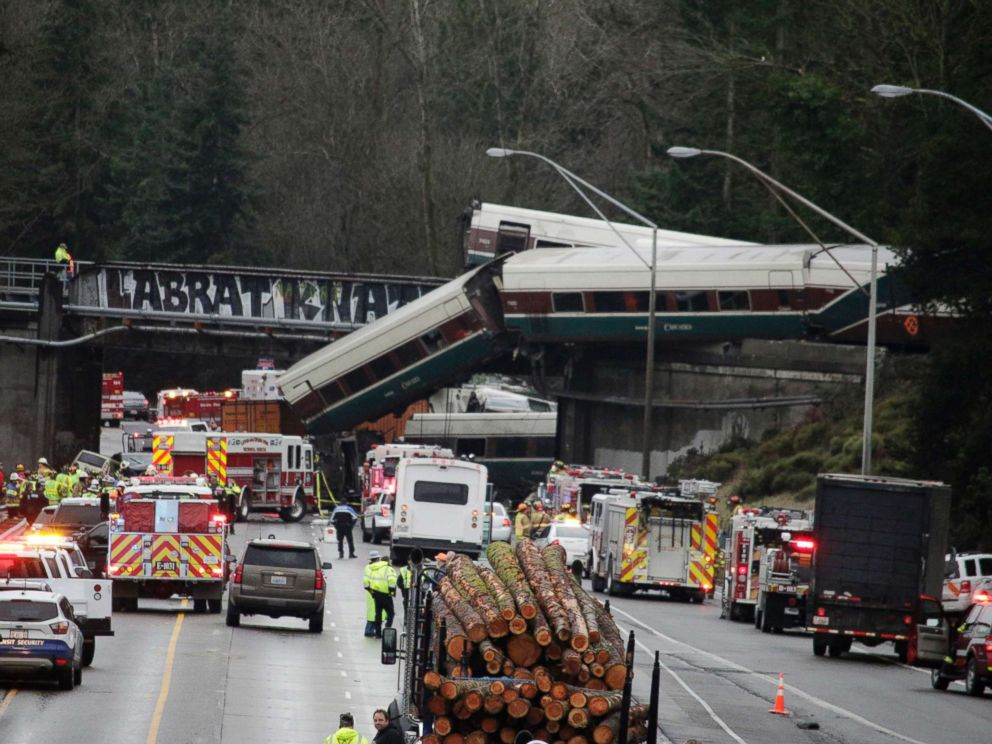
\includegraphics[width=5in]{TitleImage.png}\\
    %citation
    (Rachel La Corte/AP)
}
\author{Michael Wu, Doruk Karınca, Austin Olson,\\Christian Clarion, John Song}
\date{Engineering 183EW: Engineering and Society \\ Discussion 1G \\ March 19, 2018}

\makeglossaries

\newacronym{ptc}{PTC}{Positive Train Control}
\newacronym{ntsb}{NTSB}{National Transportation Safety Board}
\newacronym{fra}{FRA}{United States Federal Railroad Administration}
\newacronym{usdot}{USDOT}{United States Department of Transportation}
\newacronym{rsia}{RSIA}{Railroad Safety Improvement Act}
\newacronym{gps}{GPS}{Global Positioning System}
\newacronym{wmata}{WMATA}{Washington Metropolitan Area Transit Authority}
\newacronym{metrolink}{Metrolink}{Southern California Regional Rail Authority}
\newacronym{abs}{ABS}{Automatic Block Signaling}
\newacronym{cbtc}{CBTC}{Communications Based Train Control}
\newacronym{eatc}{E-ATC}{Enhanced Automatic Train Control}
\newacronym{ats}{ATS}{Automatic Train Stop}
\newacronym{atc}{ATC}{Automatic Train Control}
\newacronym{itcs}{ITCS}{Incremental Train Control System}
\newacronym{icscert}{ICS-CERT}{U.S. Industrial Control Systems Cyber Emergency Response Team}
\newacronym{ddos}{DDoS}{Distributed Denial of Service}

\patchcmd{\tableofcontents}{\contentsname}{\MakeUppercase\contentsname}{}{}

\begin{document}

\pagenumbering{Alph}
\maketitle

\frontmatter
\tableofcontents
\listoffigures
\listoftables

\mainmatter
\section{Executive Summary}

On May 12, 2015, an Amtrak passenger train in Philadelphia entered a 50 mph
curve at 108 mph. The train derailed, leaving eight people dead and nearly two
hundred injured. Safety reports determined that an existing technology known
as \gls{ptc} could have prevented this incident.

Because of the vital role trains have played in American life for two
centuries, train safety is a paramount concern. Either on short trips to work
or long trips across the country, a vast number of people ride on trains
everyday: Amtrak alone estimated their passengers as numbering 31.3 million in
2016. The \gls{ntsb} and the \gls{fra} are two of the most
important government bodies for the purpose of train safety.

In recent years, many fatal crashes have placed a more immediate emphasis on
train safety. Various crashes in Massachusetts, New York, Washington D.C.,
Philadelphia, and California brought attention to an important new technology:
\gls{ptc}. \gls{ptc} is a backup system designed to apply the brakes in the
case of driver error. All of the train crashes mentioned were caused by human
error; the engineers driving the locomotives were distracted, tired, or simply
unprepared. Upon review by the \gls{ntsb} and other agencies, it was
determined that \gls{ptc} could have prevented each of these accidents from
happening.

\gls{ptc} is an automated software-based system. The primary design premise is
that trains should be able to recognize unsafe driving behavior and correct it
by applying the brakes. There are many things for the software to consider in
determining this unsafe behavior. One of them is determining if a collision
will take place. For example, if a train is approaching a stretch of track
already occupied by another train, the control system can notify the engineer
of the problem. If the issue is not corrected in time, the control system can
remotely apply the brakes to the approaching train to prevent the collision.
\gls{ptc} can also reduce a train’s speed if it is approaching a length of
track at an unsafe speed. In the Philadelphia crash mentioned above, the
\gls{ntsb} safety report concluded that \gls{ptc} could have prevented this
accident from happening. Numerous other recent crashes have underscored the need
for active \gls{ptc} as soon as possible.

\gls{ptc} technology utilizes several different systems to make its decisions.
\gls{gps} devices onboard each train, as well as other fixed-block devices
such as track circuits and axle counters, pinpoint the exact location of each
train moment by moment. Onboard technology can determine a train’s speed and send
this information to the central control system. \gls{ptc} software then generates
signals; these can be either permissive (suggested) or absolute (required) for
the train engineer to carry out. The system can intervene by applying the
brakes if this is not done hastily enough. Cab signaling systems transmit
signals to train engineers automatically, reducing the possibility that
wayside signals (such as signs on the side of the tracks) will be missed.
Redundant systems throughout the entire \gls{ptc} system further decrease
accident probability. \gls{ptc} thus helps to eliminate accidents due to
train-to-train collisions, overspeeding, improperly aligned switches, and
incursion into work zones without proper authorization.

The \gls{fra} has been attempting to institute widespread \gls{ptc} since
1990. However, it was not until 2008 that Congress passed an act mandating its
implementation. The \gls{rsia} of 2008 placed a 2015 deadline for railway
companies to have operational \gls{ptc} on all tracks. However, when railway
companies complained that \gls{ptc} implementation was too expensive, Congress
granted them an extension until the end of 2018 with the possibility of
another extension through 2020. Most companies are now making significant
progress, but some are still lagging behind schedule. The economic costs of
\gls{ptc} are extremely high, so Congress has set aside \$6.6 million each
year to help railway companies with implementation. This is far from enough to
seriously expedite the process, and most railway companies will need the
additional deadline extension through 2020.

Several technical challenges arise in \gls{ptc} implementation. It’s possible,
and even probable, that \gls{ptc} will negatively affect performance. By
restricting motion by applying the breaks, railway capacity  will decrease.
Component degradation, which is unavoidable, must be graceful so that the
system can be repaired easily and relatively cheaply. Finally, in order to be
fully robust, \gls{ptc} systems must be interoperable; with a plethora of
railway companies in the country, it is vital that they are eventually able to
function together effectively.

In addition to the technical challenges of \gls{ptc}, there are also some
ethical and societal considerations to draw from in analyzing \gls{ptc}. The
most important hindrance of timely \gls{ptc} implementation is the
insufficiency of funding for its research and development. The funding that
the federal government provides to local authorities is in the scale of tens
of millions of dollars, whereas ungenerous budget estimates of \gls{ptc}
implementation is in the scale of billions of dollars. Therefore there is a
need for a significant source of funding.

The main reason for \gls{ptc}’s high price tag is the cost of researching and
developing the technology. Given that Union Pacific has a successful
implementation of \gls{ptc} in 98\% of its infrastructure, we recommend that
Union Pacific open-source its \gls{ptc} technology for the use of other
railways. We derive from duty ethics in analyzing this ethical dilemma.

Another concern is the safety and reliability issues associated with making a
\gls{ptc} system that delivers the desired protection from fatal crashes. Experts
observing the \gls{ptc} development practices have identified
security vulnerabilities that can be used to disrupt and hijack the \gls{ptc} system,
potentially causing worse crashes than the ones that we intended to prevent.
Our recommendation in this case is to err on the side of caution, leaning towards a
slower but secure development of \gls{ptc} than develop it
posthaste. We derive from utilitarianism in the making of this decision.

We will also address concerns related to labor displacement. There is a
misconception that \gls{ptc} will automate all types of train motion and
render the engineer obsolete. However, \gls{ptc} is merely an automatic
braking system: it identifies a potential for derailment or crash and applies
the brakes if the brakes are not applied by the engineer in a timely manner.
In fact, development efforts of \gls{ptc} results in adding more jobs to the
labor economy. Union Pacific has invested over \$2 billion and hired about a
%citation
thousand engineers to work on the development of \gls{ptc} (Union Pacific, 2018).
Therefore a discussion on the negative impact on labor economy is unfounded.

Finally, we discuss the legislative issues with \gls{ptc}, namely, Congress’
stance in the legal enforcement in \gls{ptc}. Deadline extensions for railway
companies to implement \gls{ptc} have totaled to 5 years and are expected to
increase. Rights ethics is summoned to analyze the actions of the Congress and
its responsibility to U.S. citizens. Essentially, the people’s rights to life
and safety are put at risk, therefore Congress needs to be steadfast in its
enforcement of deadlines.

This analysis shows that implementation of \gls{ptc} is a multifaceted process
with difficulties in both technological and societal viewpoints. Our use of
various ethical frameworks helps bring structural meaning to decision-making
processes and advocate for the decisions that uphold ethical values we all can
stand for.

\pagebreak

\section{Introduction}

In preparing this report we initially divided our research between broad aspects
of our topic. John and Michael decided to research the technological aspects of
\gls{ptc}, Doruk researched the economics behind \gls{ptc}, Austin researched the
laws regarding \gls{ptc}, and Christian examined train crashes that could have
prevented by \gls{ptc}. After compiling sufficient information, we wrote short
descriptions of our research individually. At this point, we had not yet received
the course survival guide, and had no idea what the actual objective of our
report was. In week eight of the quarter, we received the survival guide and
drafted an outline for our report. We attempted to integrate our research into
our technology and society sections of our outline. Then we brainstormed major
ethical issues that were relevant to our topic and assigned writing sections for
each group member.

We decided to include the train derailment cases that Christian researched in the
background, John and Michael’s technical research in the technological issues
section, and Austin and Doruk’s economic and legislative research in the ethical
and societal issues section. For each ethical issue, we applied ethical
frameworks to justify our reasoning about which course of action should be taken.
Each member of our group discussed our ethical analysis with each other. We tried
to separate our ethical analyses so that the person who researched an ethical
issue the most provided analysis for that issue. Afterwards, we drew conclusions
based on our ethical analysis and wrote recommendations for action.

Our editing process was done in person, and we met for a period of about six to
seven hours as a group to finalize this report. During this time period, we integrated
our work, wrote additional sections required for the final report such as the summary,
introduction and conclusion, and worked to improve the flow between sections. After
completing the bulk of our writing, we added images and diagrams to
help expand on our topic, some of which we drew ourselves. We also compiled a glossary
and table of contents.

Shown below is our contribution matrix, where X indicates primary contribution.

\begin{table}[htbp]
    \begin{center}
        \caption{Responsibility Assignment Matrix}
        \begin{tabular}{r|c c c c c }
            & Doruk & John & Christian & Michael & Austin\\
            \hline
            Formatting & X & X & & X & \\
            Executive Summary & X & & & & X \\
            Introduction & & & & X & \\
            Background & & & X & & X\\
            Technological Issues & & X & & X & \\
            Ethical and Societal Issues & X & X & X & X & X\\
            Recommendations & & & X & & X\\
            Conclusion & X & & & X & \\
        \end{tabular}
    \end{center}
\end{table}

\clearpage
\pagebreak

\section{Background}

Train accidents are devastating for the victims and their families: in the past
decade there have been 20 railroad incidents across the United States, causing
%citation
147 fatalities in the past decade alone (U.S. Dept. of Defense, 2017). Many of these
accidents were collisions or derailments caused by human
operator error and could have been prevented with technology known as \gls{ptc}.
\gls{ptc} is a system which uses sensors on trains and on tracks to automatically
stop a train when a potentially dangerous situation is present. The system is
designed to prevent speeding derailments, train-to-train collisions, and
work-zone incursions. Over the past decade, it ``could have prevented at least 23
deaths and 300 injuries'' according to \gls{ntsb} chairman, Robert Sumwalt
%citation
(Dooley, 2018). By implementing \gls{ptc} across the country, people will have
more faith in our infrastructure and lives will be saved. Most of these crashes
could have been prevented because human error was the root source of the
catastrophic crashes.

\subsection{Case Studies}

By analyzing the deadliest train incidents of the past decade, it becomes
apparent that many of these collisions are very similar and that human negligence
and failure or outdated technology is the root of most collisions. The six
incidents with the worst casualties are listed below.

\begin{enumerate}
    \item
    \begin{itemize}
        \item \textbf{Where}: May 28, 2008 in Newton, Massachusetts.
        \item \textbf{Casualties}: 1 killed; 6 injured.
        \item \textbf{What}: The accident occurred between two westbound
        Massachusetts Bay Transport Authority trains, since the operator of one
        train, Train 3667, failed to stop at a red signal and accelerated to a
        maximum authorized speed of 38 mph and collided with an already stopped
        train, train 3681. The operator of  of train 3667 died from blunt force
        trauma and was the only fatality while six others were injured. The total
        damage was estimated to be \$8.6 million dollars.
        \item \textbf{Why}: According to the \gls{ntsb}’s report on the incident,
        the operator failed to recognize the stopping signal. This was most
        likely due a loss of awareness from micro-sleep, a brief episode of sleep
        lasting between a fraction of a second and 30 seconds that can occur in
        anyone suffering from ``fatigue or inadequate sleep''.
        \item \textbf{Preventable}: Yes, according to the \gls{ntsb} report,
        ``This accident in Newton, Massachusetts, is another in a long series of
        accidents that could have been prevented the territory been equipped with
        %citation
        a positive train control system'' (NTSB Newton, 2009).
    \end{itemize}
    \item
    \begin{itemize}
        \item \textbf{Where}: September 12, 2008 in Chatsworth, California.
        \item \textbf{Casualties}: 25 killed, 102 injured.
        \item \textbf{What}: A \gls{metrolink} passenger train collided head-on
        with a Union Pacific Railroad freight train. The \gls{metrolink}’s
        locomotive and one of the three passenger cars derailed while two of the
        %citation
        freight’s locomotives derailed and 10 of its 17 cars derailed (Hanna and Criss,
        2018). Damages were in excess of \$12 million.
        \item \textbf{Why}: The cause of the accident was the failure of the
        \gls{metrolink} engineer to appropriately respond to a red signal which
        led to the head on collision with the Union Pacific Railroad train. The
        engineer failed to respond accordingly because of use of a wireless
        device. During the time periods that the engineer was responsible for
        operating the train, he sent 21 messages and received 20 while also
        making 4 outgoing telephone calls. This is a violation of The General
        Code of Operating Rules.
        \item \textbf{Preventable}: Yes, the final investigation report that the
        %citation
        use of \gls{ptc} would have prevented the crash (NTSB Chatsworth, 2010).
    \end{itemize}
    \item
    \begin{itemize}
        \item \textbf{Where}: June 26, 2009 in Washington D.C.
        \item \textbf{Casualties}: 9 killed; 52 injured.
        \item \textbf{What}: \gls{wmata} train 112 collided into the back of
        train 214, which was stopped on the tracks. The back car of train 214
        telescoped about 63 feet into the lead car of train 112. Damage to train
        equipment exceeded \$12 million.
        \item \textbf{Why}: A track circuit component meant to detect trains
        failed where train 214 was stopped. Train 214 was essentially invisible
        to train 112 and train 112 was commanded to continue going into the back
        of train 214.
        \item \textbf{Preventable}: Yes, \gls{wmata} was using an outdated system
        of a train control system known as the automatic block system which
        implements on track circuits to record where trains are located so that
        only one train can occupy a block at a time. \gls{ptc} would have
        prevented this accident since it relies on \gls{gps} and wireless
        communication.
    \end{itemize}
    \item
    \begin{itemize}
        \item \textbf{Where}: December 1, 2013 in Bronx, New York.
        \item \textbf{Casualties}: 6 killed; 61 injured.
        \item \textbf{What}: The Metro-North Railroad passenger train derailed at
        a left-hand curve. Damages exceeded \$9 million.
        \item \textbf{Why}: The train derailed because the train was moving 82
        mph, significantly faster than the imposed maximum speed of 30 mph. The
        operator responsible had recently complained about fatigue due to his
        shift schedule which likely caused his lack of awareness when changing
        the speed of the train to make the turn.
        \item \textbf{Preventable}: Yes, The \gls{ntsb} report states that the
        %citation
        implementation of \gls{ptc} could have prevented this incident (NTSB Metro North,
        2014).
    \end{itemize}
    \item
    \begin{itemize}
        \item \textbf{Where}: May 12, 2015 in Philadelphia, Pennsylvania
        \item \textbf{Casualties}: 8 killed; 185 injured.
        \item \textbf{What}: Amtrak passenger train 188 derailed going 106 mph
        around a curve that was restricted to 50 mph. Damages exceeded that of
        \$31 million.
        \item \textbf{Why}:The accident was likely due to the operators loss of
        situational awareness since he likely do not intend to accelerate the
        train to 106 mph. While operating the train, the operator, who was found
        to have a regular and healthy sleep schedule and never found to use his
        phone, was distracted by a conversation about an emergency on another
        nearby train where the window of a Septa train shattered which sent glass
        into the eye of that engineer. This conversation occurred between 9:13
        and 9:19 PM and the derailment occurred at 9:21 PM. The operator admitted
        in an interview three days after the incident that he was distracted by
        the conversation and was worrying about his own safety since he was
        travelling in a nearby area.
        \item \textbf{Preventable}: Yes, contributing to the cause was the ``lack
        %citation
        of positive train control system'' (NTSB Philidelphia, 2016).
    \end{itemize}
    \item
    \begin{itemize}
        \item \textbf{Where}: December 18, 2017 in DuPont, Washington.
        \item \textbf{Casualties}: 3 killed; over 100 injured.
        \item \textbf{What}: An Amtrak passenger train derailed on its inaugural
        journey, sending 13 of its 14 cars off an overpass and onto rush hour
        traffic below.
        \item \textbf{Why}: The train was travelling 80 mph in a 30 mph zone. The
        train engineer told \gls{ntsb} reporters that he mistook a signal and
        only braked moments before the crash.
        \item \textbf{Preventable}: Most likely, this incident is still being
        %citation
        investigated by the \gls{ntsb} (Hanna and Criss, 2018).
    \end{itemize}
\end{enumerate}

\begin{figure}[ht]
    \begin{center}
        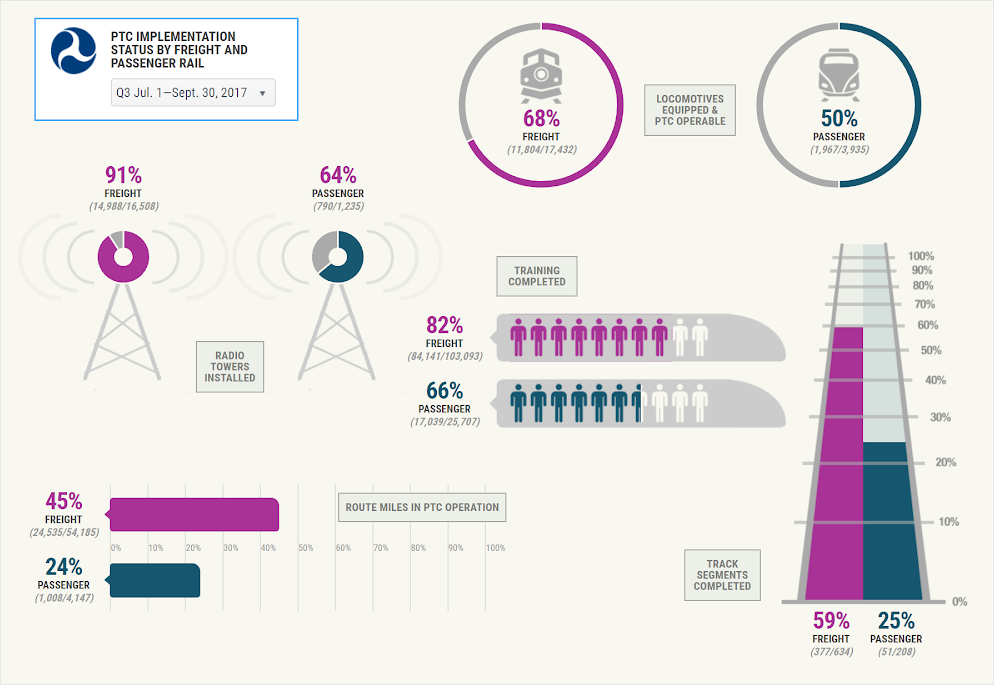
\includegraphics[width=\textwidth]{PTCAdoption.png}
        %citation
        \captionsetup{justification=centering}
        \caption[National PTC Adoption]{Total national \gls{ptc} adoption progress as
        of September 30, 2017 (FRA PTC Implementation, 2017).}
        \label{adoption}
    \end{center}
\end{figure}

\subsection{Current Adoption}

With the implementation of \gls{ptc}, these lives would have been saved. The lost
lives cannot be brought back, but if \gls{ptc} becomes universally implemented as
soon as possible, then further casualties will be prevented. Unfortunately,
however, most train companies have yet to fully install \gls{ptc}, putting
additional lives at risk. According to the \gls{fra}, as of September 30, 2017,
only 64.4\% of freight locomotives and only 43.8\% of freight route miles in
America are equipped with operable \gls{ptc}; as for just passenger trains, only
%figure
50\% of locomotives and 24\% of route miles have \gls{ptc}; see Figure
%citation
\ref{adoption} (FRA PTC Implementation, 2017).

\subsection{Legal Coverage}

Since train derailment due to driver error is such a common issue, laws have been
passed to mandate the use of \gls{ptc}. \gls{ptc} had been listed in the ``Most
Wanted List of Transportation Safety Improvements'' by the \gls{ntsb} since 1990
%citation
(NTSB Most Wanted, 2007). However, no law was passed
regarding it until 2008, nearly twenty years later. In October 2008, Congress
passed Public Law 110-432: the \gls{rsia}. Many topics were addressed in this
program, including railroad worker hours, standards for track inspection, and
certification of locomotive conductors. However, the mandatory implementation of
\gls{ptc} was the most important part of this act. The \gls{rsia} required a plan
of action from all railroads, provided technical assistance to accomplish
\gls{ptc}, demanded a 2012 progress report, and allowed Congress to penalize
companies not complying with the laws. The \gls{rsia} also included provisions to
provide economic and logistical assistance to railroads implementing \gls{ptc}: a
large loan, many grants, and a dedicated \gls{ptc} task force to monitor and
%citation
assist the rail companies (Congress, 2008). The governing body in charge of this
process, the \gls{fra}, is a subdivision of the \gls{usdot}.

\subsection{Deadline Extensions by Congress}

Initially, the \gls{rsia} deadline for \gls{ptc} implementation was December 31,
2015. When several major rail companies appeared to be behind schedule and asked
for more time to install the necessary technology, Congress voted to move this
deadline back to December 31, 2018. In the same extension, they included a
possibility of a further extension through 2020 if railroad companies met certain
requirements but needed still more time to finish \gls{ptc} implementation.

The possible 2020 extension is based upon several criteria. Each railroad must
give written notification that they have completed these steps to the \gls{fra}
in order to be granted the extension and avoid daily \gls{fra} fines. By the end
of 2018, railway companies must have installed all \gls{ptc} hardware. They must
have implemented \gls{ptc} on a majority of territories and have made sufficient
progress on employee training. Finally, the companies must submit a revised
\gls{ptc} Implementation Plan to the \gls{fra} to be fully \gls{ptc} compliant by
the end of 2020. As of September 30, 2017 (the most recent available data), many
companies are making substantial progress toward these goals, yet they will likely
%table
need the additional deadline extension. Table \ref{progress} shows individual
railway progress toward total \gls{ptc} integration.

\begin{table}[ht]
    \begin{center}
        %citation
        \captionsetup{justification=centering}
        \caption[Individual PTC Implementation Progress]{Individual railroad progress
        toward \gls{ptc} implementation as of\\
        September 30, 2017 (FRA Individual PTC Progress, 2017).}
        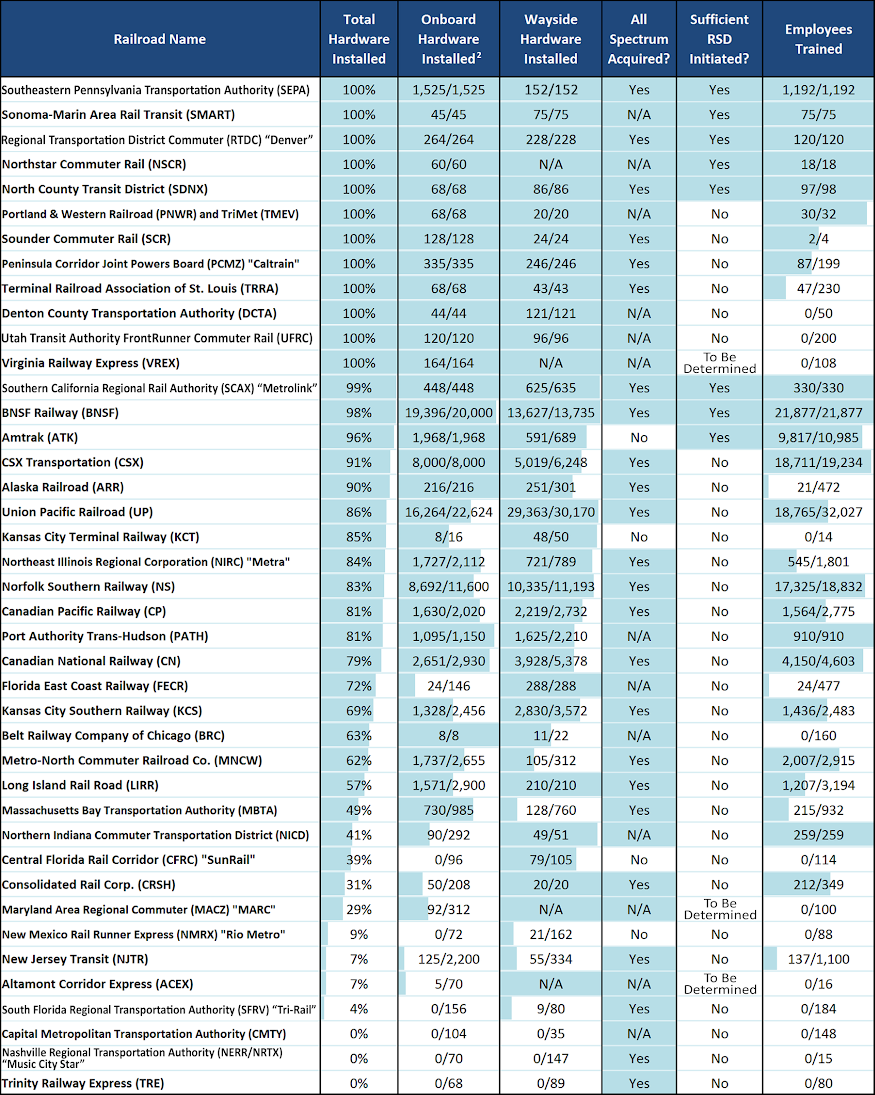
\includegraphics[width=0.9\textwidth]{RailroadProgressTable.png}
        \label{progress}
    \end{center}
\end{table}

\clearpage
\pagebreak

\subsection{Progress So Far}

The \gls{rsia} requires many \gls{ptc} components to be completed by all
railroads: locomotive equipment, track segments, radio towers, employee training,
and a \gls{ptc} safety plan. These components must all be completed at the same
location for a route mile to be considered ``in \gls{ptc} operation''. The
\gls{fra} has progress reports for all rail companies operating within the U.S.
Amtrak, one of the most popular passenger railways in the country, has indeed made
progress to complete implementation of \gls{ptc}: 67\% of its route miles are in
operation, and more than 70\% of locomotives equipment, radio towers, and training
has been completed. In fact, the section of track where the deadly 2015
Philadelphia train crash occurred had the proper equipment installed. However,
Amtrak had not conducted the tests needed to switch the system on. The accident
was a result of human error and a lack of \gls{ptc}, eight people were killed and
an additional 185 were injured. Many other railroad companies are lagging behind
Amtrak in \gls{ptc} implementation, including multiple railways which have made no
progress at all towards these goals.

\pagebreak

\section{Technological Issues}

\subsection{Basics of Railroading}

The goal of train traffic control involves both \textit{protection}, which ensures
separation of trains and prevents conflicting movements that may lead to a
collision, as well as providing additional control over the timing of movements in
%citation
order to encourage \textit{efficiency} (Bryan and McGonigal, 2006). As a mode of
transportation, railroads are very different from cars or airplanes which gives
them different kinds of safety issues:

\begin{enumerate}
    \item \textit{Excessive speed} can cause a train to lose control and derail.
    This is especially true on curved tracks, where the rails may not be able to
    handle the large centrifugal force of a turning train. Enforcing speed limits
    can solve this problem.
    \item Because trains run on rails and cannot easily maneuver, train drivers
    can control the speed of a train but not its direction. Trains also tend to be
    heavier and have a much larger stopping distance. In many cases, it is already
    too late to stop a train when an obstacle comes into view. Because of this,
    \textit{movement conflicts} are much more dangerous. Trains must be carefully
    scheduled to avoid head-on and rear-end collisions, as well as collisions at
    crossings.
    \item In addition, railroad junctions are controlled by switches, which are
    mechanical devices that control the turning direction of a train. A switch
    must fully move into place in order for a train to proceed in either
    direction. A switch can be \textit{misaligned} and cause a train to derail if
    it is not in any of these set positions. In addition, switching a train onto a
    wrong track can lead to collisions and overspeed conditions. We will refer to
    these two conditions collectively as \textit{improperly aligned switches}.
    \item \textit{Mechanical failure} of the rail, car wheels, or brakes, as well
    as obstruction of the tracks, can lead to derailments and collisions. These
    failures can be caused by design defects as well as improper maintenance
    procedures.
\end{enumerate}

Railroad companies must work to solve these problems before attempting to increase
operational efficiency, or trying to safely schedule as many trains as possible.
These two goals are often at odds. Scheduling trains more often can increase
efficiency, but this leads to reduced spacing between trains and an increased
chance of a collision. Because of this, train control often involves a
comprehensive coordination between multiple operating segments, each responsible
for different functions: \textit{detection}, \textit{processing},
\textit{communication}, and \textit{enforcement}. The first three together are
often known simply as \textit{signaling}. A typical division of labor looks like
%citation
the following (Association of American Railroads, 2018):

\begin{enumerate}
    \item \textit{Wayside} and {onboard} segments, consisting of personnel and
    equipment that sense and controls train movement:
    \begin{enumerate}
        \item The wayside segment consists of track-side equipment and personnel,
        including equipment that monitors track conditions and occupancy, as well
        as switches that divert movement.
        \item The onboard segment consists of the train crew, sensors that
        determine the status of a train, and enforcement devices.
    \end{enumerate}
    \item The \textit{central office} (a.k.a. \textit{back
    office}/\textit{dispatching}) segment makes use of the collected information
    to direct movement.
\end{enumerate}
Operations on any of the above segments can take place at various levels of
automation. They can range from being entirely dependent on manual operation,
manually operated with an automated system as an emergency fallback, or even fully
automatic.

Together, these segments perform the functions of detection, processing,
communication and enforcement. Even though responsibility for controlling
communication is typically distributed among segments, the most technically
challenging aspect is the communication between ground stations and the moving
train. We will focus on this aspect in the following discussion.

\subsection{Signaling Technologies}

\subsubsection{Detection}

Many methods exist to determine which train occupies which stretch of track. The
earliest systems relied on verbal communication between train operators to
establish occupancy of a block, as well as the location of individual trains
%citation
(Bryan and McGonigal, 2006). Later, more automated detection systems came along.
These systems are further divided into \textit{wayside-centric} or
\textit{train-centric} systems.

In a wayside-centric system, devices installed along the tracks are responsible
for detecting the presence of a train. These devices, such as track circuits and
axle counters, can determine occupancy for fixed stretches of track. These
sections of track are known as blocks, and wayside signals form the backbone of
%citation
\textit{fixed-block} signaling systems (Pascoe and Eichorn, 2009). Although track
circuits do not directly identify individual trains, this data can be combined
with information about when and where a particular train departs and arrives to
infer its location.

By contrast, in train-centric detection, the train itself is responsible for
collecting its location data. Automatic positioning of individual trains can be
performed with the assistance of transponder systems installed along tracks. When
a train passes over a transponder, the device is activated and sends its location
to the train. Positioning can also happen via other means, such as by using
\gls{gps}. Typically, the location signal is first received by onboard devices,
which then transmit it to a dispatch center. In practice, these absolute
positioning devices are only activated intermittently because they are
supplemented by devices that collect relative location data such as speed or
acceleration. Therefore with train-centric detection, a train’s location can be
known with more precision than by using fixed-block methods. This forms the basis
%citation
of \gls{cbtc}, which is a more modern form of train control (Pascoe and Eichorn,
2009).

Train control systems also use other types of data to ensure safety. Onboard train
equipment can collect speed information that is used to enforce speed limits.
Also, track-side devices can detect safety hazards on the tracks. For example,
some track circuit systems can provide limited detection of broken track rails
which disconnect the circuit. Similarly, slide fences\textemdash barriers which
form electrical circuits that are easily broken or displaced\textemdash are used
to detect falling rocks. Other types of devices detect overheating wheels and
%citation
brake problems, which when untreated can cause a train to derail (Bryan and
McGonigal, 2006).

\begin{figure}[ht]
    \begin{center}
        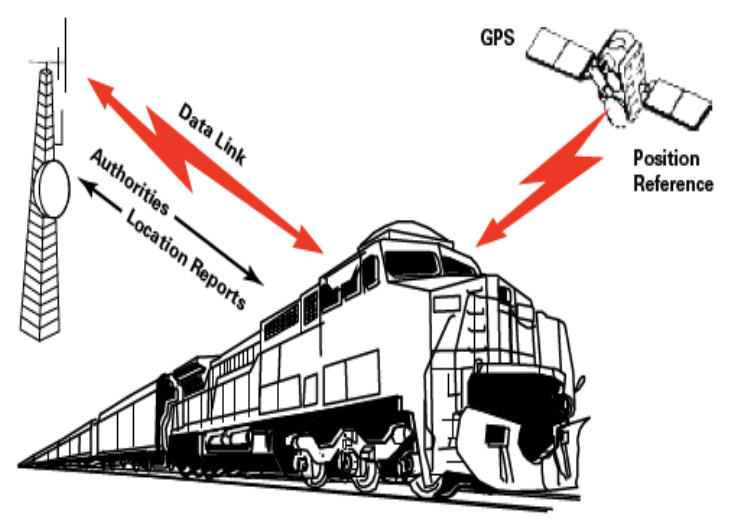
\includegraphics[width=4in]{PTCDiagram.png}
        %citation
        \caption[GPS-Based Train-Centric Positioning]{Implementation of \gls{gps}-based
        train-centric positioning (Badugu and Movva, 2013).}
    \end{center}
\end{figure}

\subsubsection{Authority Generation}

Given that trains move on predetermined tracks, more precise prediction of their
positions over time is possible as opposed to a self-driving car on a free road
where the next course of action is less deterministic. This paves the way for
dispatching systems in which we coordinate multiple trains in the same railroad
system.

The earliest form of train dispatching heavily relied upon timetables, which
specified in advance where trains should be at key moments in time. These systems
were not very flexible, and often had to be augmented by additional communication
in order to cope with delays, breakdowns and other ``unforeseen circumstances''
%citation
(Bryan and McGonigal, 2006).

More sophisticated dispatch operations are based on the dynamic generation of
movement authorities. These authorities are permissions for a train to proceed
%citation
through a block (Lindsey, 2009). For safety reasons, these blocks are made long
enough so that trains have enough space to stop before reaching the end. The use of
dynamic movement authorities allows for more flexible and efficient train control.

%citation
In addition, authority generation can be discrete or continuous (Pascoe and Eichorn,
2009). As the names suggest, the former is based on fixed section of railroad
tracks while the latter works arbitrary sections of rail. These lead to two
signaling systems known as fixed-block signaling and moving-block signaling,
respectively. In these systems, only one train is allowed to occupy a block at a
time. If a train attempts to move into a block that is already occupied, operators
signal for the train to stop until the block becomes vacant again.

Signals that indicate authority can either be permissive or absolute. Permissive
signals focus on protection, whereas absolute signals also focus on efficiency. The
dispatch process can be fully manual, in which an operator would be physically
responsible for pulling the levers that control the switches and signal
indications. This process can be augmented by a mechanical or computer-assisted
%citation
conflict checking device to protect against human error (Lindsey, 2009). It is
typically done in a control center, but sometimes track-side equipment also
%citation
generate permissive signals, which are used as a fallback (Bryan and McGonigal,
2006).

\subsubsection{Delivery}

Once the movement authorities are generated, they need to be communicated to the
train crew and onboard equipment. Communication can be accomplished in a fully
manual fashion, in which dispatchers would issue verbal instructions to the train
crew in person or over radio. More mechanized systems such as wayside signaling are
also commonly used. This method uses fixed track-side equipment that provides
direct visual indication to the onboard crew. In addition to movement authorities,
the train crew also need to know about speed restrictions, which can vary based on
track maintenance conditions. Traditionally, this was accomplished using verbal
%citation
communication and/or speed limit signs installed along the tracks (Pascoe and
Eichorn, 2009).

\begin{figure}[ht]
    \begin{center}
        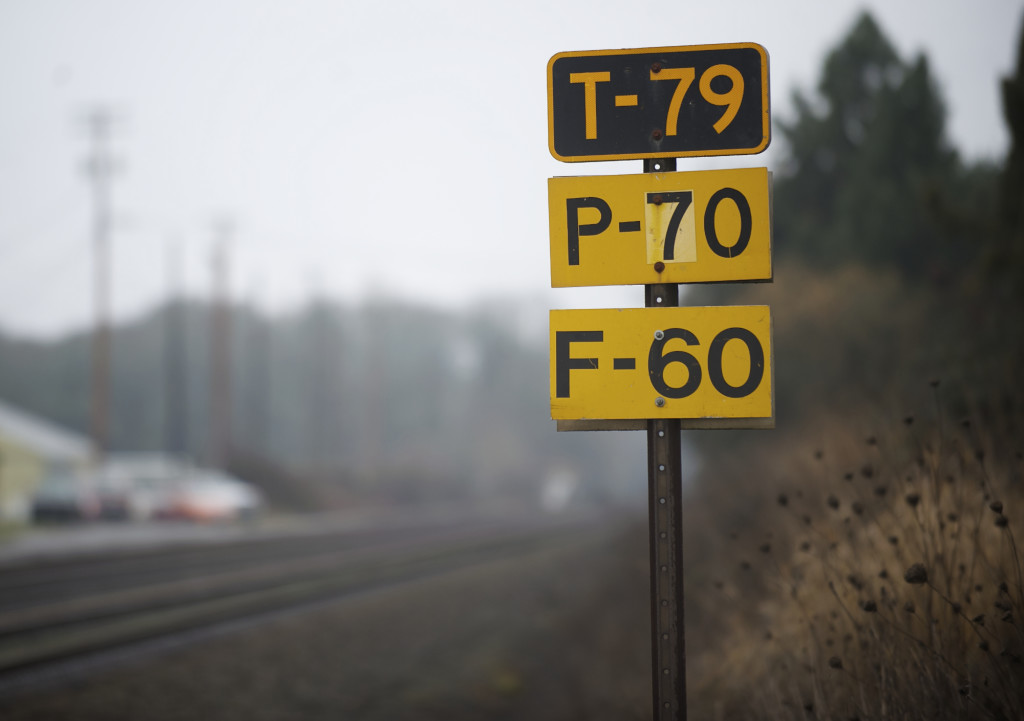
\includegraphics[width=4in]{SpeedLimits.png}
        %citation
        \caption[Speed Limit Sign]{A speed limit sign (Graf, 2013).}
    \end{center}
\end{figure}

In contrast, \textit{cab signaling} relies on electromagnetic means such as
magnetic induction or radio to transmit signals and speed limit information, giving
it numerous advantages over wayside signaling. Signals will be shown on an onboard
display, which is convenient for train drivers as they no longer have to rely on
spotting wayside signals. Additionally, they do not need to worry about
%citation
accidentally missing a signal, as happened in the Dupont derailment (NTSB Washington State, 2018).
Cab signals can be easily processed by other onboard equipment that performs automatic
enforcement, providing more sophisticated protection against human error. In
addition, this can help reduce costs for track-side equipment because the same
transponder systems used for detection can be used for signaling as well. Cab
signaling can either replace wayside signaling or function alongside it as an
additional protective measure (Bryan and McGonigal, 2006).

\subsection{Signaling Systems}

We have examined the individual technologies required to perform some basic
functions: detection, processing, communications, and enforcement. These
technologies combine to form train control systems. We will now look at these
systems, first from the perspective of signaling. Then we will consider how
enforcement technologies interact with the rest of the system.

\begin{figure}[ht]
    \begin{center}
        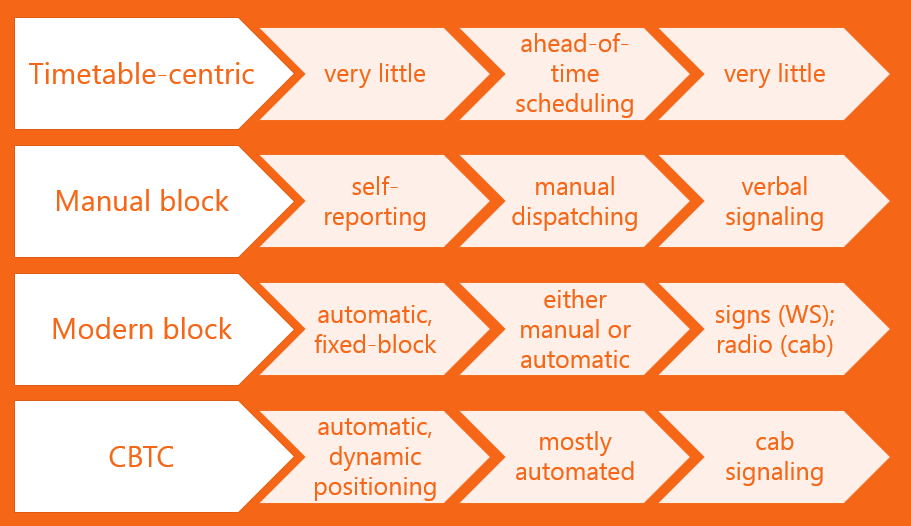
\includegraphics[width=4in]{SignalingTechnologies.png}
        \caption{Overview of signaling technologies.}
    \end{center}
\end{figure}

\subsubsection{Manual Signaling}

Early train traffic control systems were largely manual. Examples include the
manual block system, in which human operators would set wayside signals. Another is
the track warrant control system, where a train crew is responsible for reporting
its location to a dispatcher. The dispatchers grant authority for movement over
radio or phone. Although these systems could operate safely, they were also
inefficient, prone to human error, and had limited hazard detection abilities.
Today, they are typically used on railroads that do not see a lot of traffic.

In North America, significant areas rely on the aforementioned manual systems, as
they do not have any modern signaling equipment or automatic detection systems
installed. These sections of rail are known as dark territories. As of 2012, dark
territories comprise approximately one-third of all railroad routes by length in
%citation
the United States and Canada (Raymond, Lindsey, and Pachl, 2012). One source, a 2011
%citation
presentation by the Dark Territory Working Group of the Federal Railroad
Administration, estimates the amount of dark territory in the U.S. to be even higher
at about 54\% (FRA Dark Territory, 2011).

\subsubsection{Modern Fixed-Block Signaling}

Modern fixed-block signaling, also known as \gls{abs}, originated in the early 20th
century. Instead of relying on verbal communication, it uses detection devices such
as track circuits to determine the presence of trains. These automatically operate
signals that instruct trains to proceed, stop, or proceed with caution. The first
generation of modern fixed-block signaling systems transmitted these signals as
wayside signals. Later generations introduced the use of cab signals that could
%citation
also send speed codes or profiles to the train (Morar, 2012).

The partial automation of train control provided by \gls{abs} allows for greater
capacity of trains on a given track, which leads to increased efficiency. \gls{abs}
can replace manual signaling entirely, or it might function as an additional
protective layer on top of manual signaling. In this hybrid setup, the \gls{abs}
signals create an additional level of redundancy which protects against operator
%citation
error and equipment failure (Lindsey, 2009). This comes at the cost of increased
operating and equipment expenses.

\begin{figure}[ht]
    \begin{center}
        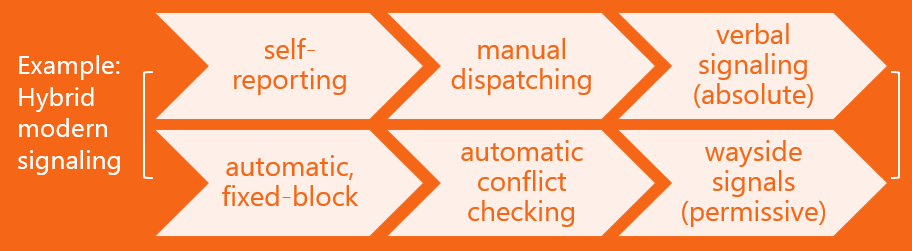
\includegraphics[width=4in]{HybridSignaling.png}
        \captionsetup{justification=centering}
        \caption[Hybrid Fixed-Block Signaling]{Hybrid fixed block signaling, with
        a manual system generating absolute signals and an automated system generating
        permissive signals.}
    \end{center}
\end{figure}

\subsubsection{Communications Based Train Control}

The newest generation of signaling systems, known as \gls{cbtc}, breaks from the
tradition of fixed block systems. \gls{cbtc} uses train-centric detection and
dispatch technologies such as transponders or \gls{gps}. It also uses a wireless
network for communication between the onboard, wayside, and office segments. This
places more responsibility on the onboard segment for detection and communication
functions, and reduces the responsibility of the wayside segment. In addition,
dispatching can be performed by an electronic system known as the zone controller.
This system can check for conflicting movements, automatically issue signals, and
manipulate track switches.

\gls{cbtc} allows for fine-grained monitoring and scheduling of trains, which can
lead to better performance. In addition, the reduced dependence on fixed mechanical
equipment can increase maintenance flexibility. However, \gls{cbtc} can also
increase the system complexity and introduce more potential safety concerns,
especially if the wireless networks are inadequately secured. As with modern block
signaling, \gls{cbtc} can either replace an older fixed-block system or function
alongside it.

Modern signaling systems are very common in North America. About half of all routes
use full \gls{abs}, \gls{cbtc}, or some combination of the two, and an additional
one-sixth use the aforementioned hybrid manual-\gls{abs} setup. Almost all European
%citation
railroads use modern signaling systems (Raymond, Lindsey, and Pachl, 2012).

\subsection{Train Protection Systems and the Technology Behind PTC}

\subsubsection{Train Protection}

Historically, human train operators have caused many deaths due to preventable
mistakes. Automated mechanisms can provide additional protection against this human
error. They can work to prevent accidents due to missed signals, movement
violations, or improperly aligned switches. Some of these systems merely provide a
warning to the train driver, while others can also perform an emergency stop
%citation
(Connor and Schmid).

These form the basis of train protection systems, which are mainly intended to
provide enforcement for train signals. One well-known protection system is based on
the trip stop, a mechanical contraption installed along the tracks at a wayside
signal. If a train passes the signal while it says to stop, the trip stop triggers
%citation
the train’s emergency brakes (Connor and Schmid). Other more sophisticated
train protection systems can guard against both movement and speed violations by
using information from the train itself.

\subsubsection{Positive Train Control}

\gls{ptc} is the modern evolution of train protection systems. As required by
federal regulations, the \gls{ptc} system must determine and prevent the following
types of safety issues:
\begin{enumerate}
    \item Possible train-to-train collisions,
    \item Overspeeding,
    \item Improperly aligned switches,
    \item Incursion into work zones without prior authorization, which can endanger
    maintenance workers as well as the train itself.
\end{enumerate}
When \gls{ptc} detects any of the above conditions, an emergency train stop will be
initiated if the train crew does not quickly act to correct the issue. In addition,
\gls{ptc} will reduce speed in places where the railway infrastructure is
%citation
considered unsafe (Government Publishing Office, 2018).

As with typical train control systems, conflict checking is done from a control
center which monitors the locations of each train in the rail system. Communication
between the control center and trains is achieved through wireless networks,
allowing a control center to cover a large number of moving trains in a given
system. The central authority issues movement authorizations for each train based
on their relative locations. If a train begins to move outside its authorized
movement zone, the control center will issue a warning to notify the train
operator, who should correct the train’s movement. If the engineer does not do so,
the control center will give a signal for the train to automatically brake.

Onboard computers store speed limit profiles for the train tracks and information
%citation
about the train’s stopping capabilities to make these calculations (Badugu and Movva, 2013).
Because this feature can be implemented onboard, constant communication with the
central authority is not necessary to enforce speed limits. The central authority
is only necessary to update stored speed limit profiles, which may be done
intermittently.

The control center can also monitor track circuits, wayside signals, and switches
on the tracks to prevent crashes. By doing so, the control center can detection
more hazards on the tracks and stop trains in more cases. However, this is an
optional part of \gls{ptc} and is not necessarily present in all \gls{ptc} systems.
\gls{ptc} cannot detect some hazards such as obstructions, flooding, or broken
rails without knowledge of track circuits.

\subsubsection{What PTC is Not}

There has been some confusion regarding what \gls{ptc} means. Some may assume it
focuses on improving efficiency, possibly due to confusion with Precision Train
%citation
Control (Lindsey, 2009). Other sources suggest that \gls{ptc} always involves
%citation
wireless networks and \gls{gps} (Badugu and Movva, 2013). In both these cases,
\gls{ptc} is conflated with \gls{cbtc} technology. In reality, \gls{ptc} is not
required to be tied to specific types of detection and signaling technologies, as
long as they can fulfill the requirements outlined by Congress.

Different technologies such as \gls{gps} or wireless location devices along the
train tracks can be used for locating trains. This means \gls{ptc} implementations
can use newer \gls{cbtc} signaling technology, or they can be implemented on top of
%citation
traditional fixed-block signaling (Vantuono, 2016). An example of the latter is
\gls{eatc}, approved by the \gls{fra} in 2016.

In addition to this, \gls{ptc} systems that use \gls{cbtc} can be deployed alongside
a fixed-block signaling system that generates absolute signals. This architecture is
similar to that of the hybrid \gls{abs} system mentioned before. Essentially, these
systems use \gls{cbtc} to perform permissive signal generation, creating redundancy
in signaling as well as enforcement. Figures \ref{PTCwithCBTC}-\ref{PTCHybridCBTC}
show that the implementation of \gls{ptc} can take a variety of forms with
different degrees of automation and redundancy. These differences lead to different
safety and cost profiles.

\begin{figure}[ht]
    \begin{center}
        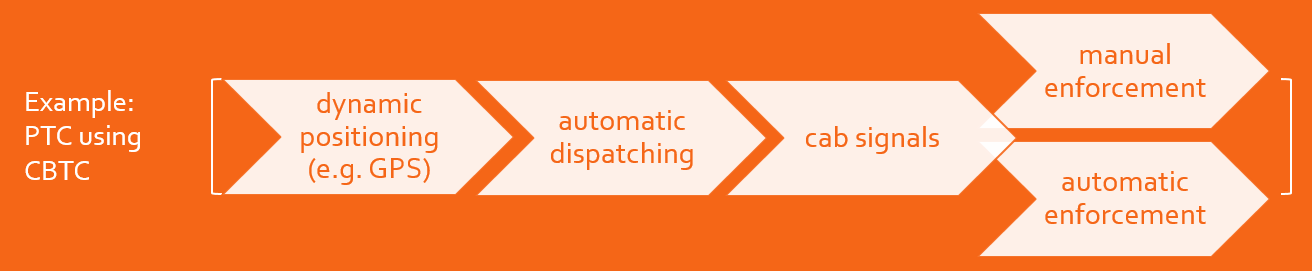
\includegraphics[width=4in]{PTCwithCBTC.png}
        \caption[PTC with CBTC]{\gls{ptc} system that completely relies on \gls{cbtc}
        and automatic dispatching}
        \label{PTCwithCBTC}
    \end{center}
\end{figure}

\begin{figure}[ht]
    \begin{center}
        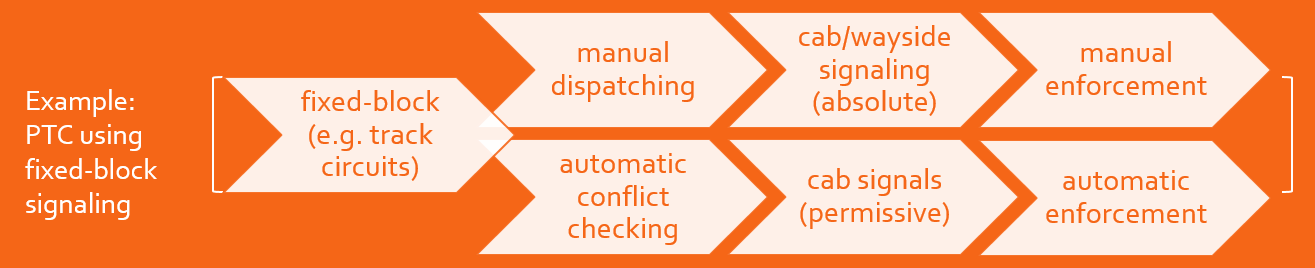
\includegraphics[width=4in]{FixedBlockPTC.png}
        \captionsetup{justification=centering}
        \caption[PTC with Fixed-Block Signaling]{\gls{ptc} system that completely
        relies on traditional fixed-block signaling, and uses manual block dispatching
        for normal operation.}
    \end{center}
\end{figure}

\begin{figure}[ht]
    \begin{center}
        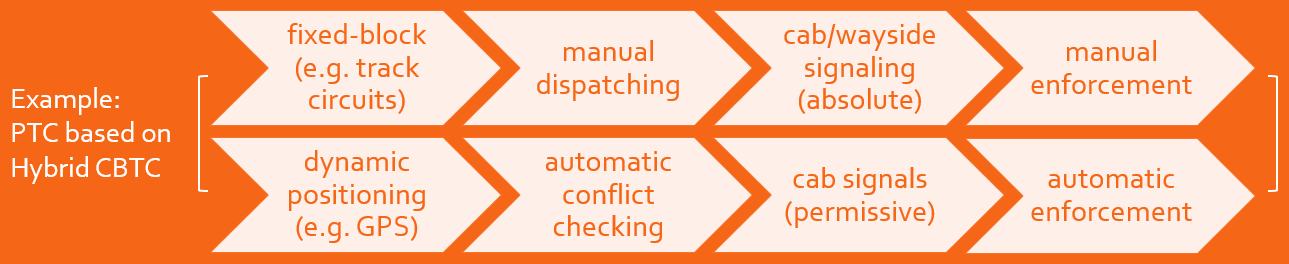
\includegraphics[width=4in]{PTCHybridCBTC.png}
        \captionsetup{justification=centering}
        \caption[PTC with Hybrid CBTC]{\gls{ptc} system using \gls{cbtc} for automatic
        signaling and enforcement, and traditional fixed-block signaling for manual
        operation.}
        \label{PTCHybridCBTC}
    \end{center}
\end{figure}

\subsubsection{PTC vs. Older Systems}

\gls{ptc} can be compared to conventional train protection systems such as
\gls{ats}. Like \gls{ptc}, \gls{ats} is defined in federal regulations
as a system that performs an ``automatic brake application'' when approaching a
%citation
block with ``restrictive block conditions'' (Government Publishing Office, 2018).
These conditions account for occupied blocks, partially
aligned switches, and excess train speed. However, \gls{ats} and \gls{ats} have
less stringent safety requirements than \gls{ptc}. For example, they are not
required to handle work zone situations. In addition, \gls{ats} and \gls{ats} are
based on fixed-block systems by definition. Compared to these older systems,
\gls{ptc} is safer and more flexible.

\subsection{Technical Challenges of PTC}

\subsubsection{Negative Performance Effects}

A concern about implementing \gls{ptc} is whether or not it will negatively affect
railway performance. Although \gls{ptc} might provide greater safety, it could also
be too restrictive and unnecessarily slow down trains. In the past, ``the freight
railroad industry has been reluctant to fit speed control devices due to the often
heavy-handed nature of such devices having an adverse effect on otherwise safe
%citation
train operation'' (Badugu and Movva, 2013). Historically, trains have relied only on signals
and human judgment to ensure safety. If trains have been operating safely this way
for decades, why limit the power of train operators who are experienced in properly
controlling their vehicles? Implementing \gls{ptc} may mean that train operators
must slow down when they know that it is safe to proceed, reducing the efficiency
of a railroad line. The \gls{fra} has recognized this challenge, and even admitted
in 2009 that ``\gls{ptc} was in fact likely to decrease the capacity of freight
%citation
railroads on many main lines'' (Badugu and Movva, 2013). Thus engineers must work to design
\gls{ptc} systems that allow for the same, or even better, levels of efficiency as
that of signaling systems without \gls{ptc}.

\subsubsection{Robustness and Reliability}

\gls{ptc} systems also need to be robust against unpredictable factors ranging from
unintended disruptions to hacking. Because \gls{ptc} relies on wireless signals for
communication between trains and a control center, it must account for these
situations. Wireless signals tend to behave inconsistently and cannot be relied
upon to be active at all times. So designers of \gls{ptc} must ensure that there
are fallbacks when wireless signals cannot be received. Using \gls{ptc} as an
additional measure on top of another signaling system ensures that there is enough
redundancy to avoid collisions even when \gls{ptc} cannot work. Additionally, the
control center must be able to identify any train that has gone offline so that it
can be brought back as soon as possible. The system must be able to tolerate broken
components and be easily repaired.

Hacking is another major issue with the development of \gls{ptc}. Engineers must
take adequate safety measures to prevent unauthorized tampering with \gls{ptc}
signals. If an attacker could falsely tell a train to stop or send false locations
signals to a control center, he could cause derailments and collisions. Railroad
technology has been vulnerable to attack in the past. In 2008, a teenager was
arrested for tampering with the streetcar system in Lodz, Poland. He had reverse
engineered the signals used to control track switches and caused derailments by
%citation
changing the switches to point the wrong way (Sweeney, 2014).

\subsubsection{Interoperability}

\gls{ptc} has various implementations, so different companies may have incompatible
\gls{ptc} systems. Because trains owned and managed by different companies often
share the same stretch of tracks, \gls{ptc} systems must be designed for
%citation
interoperability in order to function together effectively (Sweeney, 2014).
Otherwise, it could be possible that a \gls{ptc} system does not account for trains
from different companies and fails to apply brakes correctly. This could lead to
collisions that \gls{ptc} should have prevented. To avoid this, engineers should
eventually work to make \gls{ptc} compatible across all railways.

Currently a unified \gls{ptc} system is not feasible due to the state of \gls{ptc}
adoption. Some rail companies have almost completely implemented \gls{ptc}, while
others have virtually no \gls{ptc}. Additionally, rail companies would not want to
share design details for \gls{ptc} with their competitors. They have no business
incentive to do so. One way to increase \gls{ptc} compatibility across different
companies is for engineers to come up with standard operating interfaces for
\gls{ptc} systems. This makes it easier for companies to independently follow
compatible design principles.

\pagebreak

\section{Ethical and Social Issues}

\subsection{Cost and Funding}

Implementing \gls{ptc} country-wide is indeed a technical challenge, but not one
that cannot be overcome with enough money and time. The greater challenge is to
overcome the associated societal challenge, that is, find the source of money.
Having mentioned all the potential of \gls{ptc}, especially in terms of lives to
be saved, it is surprising \gls{ptc} is still open to heated debate for financial
reasons. Having covered the technological issues, we know why it will cost
billions for a system that interoperates and agrees with the standards of various
railways companies. Yet if we continue to delay implementing this, we will lose
more lives to simple human error. We mentioned that some train derailments have
been caused by something as simple as an easy-to-identify locked rail switch
%citation
or by an operator texting and overlooking wayside signals (Chatterjee, 2008). The solution
is to overcome the money barrier and support
investments that are pro-\gls{ptc}.

In any human endeavor, human error is unavoidable and should be replaced by tested
automation if possible. During the \gls{metrolink} train collision in Los Angeles,
the engineer who was texting made a human error that caused the death of 25
%citation
people (Chatterjee, 2008). This could have been prevented if an automated system to
stop the train had been in place. As mentioned in the signaling technologies
section, the fact that trains move only on predetermined tracks makes their
movements easy to identify, in contrast to something such as a self-driving car.
This makes train control a good candidate for automated control. However, even
\gls{ptc} comes with its own technical challenges: ``Railroads have had to develop
highly complex braking algorithms for both freight and passenger trains that
account for numerous factors, and not just the obvious ones like velocity, track
gradient or weight. We need to account for outside elements like weather, the
brake systems installed on different rail cars and the fact that railroads rely on
%citation
customers for cargo weight data'' (Young, 2016). Not only overcoming these
aforementioned technical challenges but also getting people together to solve such
a problem makes designing \gls{ptc} a difficult feat.

For this reason, designing \gls{ptc} is very costly which discourages railroad
companies from implementing it in a timely manner. After the above-mentioned
\gls{metrolink} accident, Congress gave railroad companies a deadline until 2015 to
implement \gls{ptc} in their lines in the \gls{rsia}. However, this deadline got
postponed to 2018. In the meanwhile, track derailments continued to take lives
%citation
(Graham, 2017). Train commuters were injured and killed in Washington because rail
companies thought that \gls{ptc} was too costly to implement on time. The main
expense of \gls{ptc} is the development operations and the research on the
technology. Development increases the costs tremendously as opposed to existing
solutions that can be simply bought from a third party, since \gls{ptc} is not a
readily-developed, commonplace technology. There are many different cost estimates
%citation
for building \gls{ptc}, ranging from \$6 billion to \$22 billion (Cullen, 2018).
This variation is due to the nonstandard type of implementation, which also suggests
how the \gls{ptc} implementation for each railway company will vary. As a result,
unpredictability of the costs makes it very difficult to set a budget. More
importantly, since the federal deadline to implement \gls{ptc} is lenient, the
project can take a while. However, projects that go overtime also go over budget,
which can add to the predicted costs.

Funding from the government could play a huge role in delivering \gls{ptc} sooner
and therefore for less money. Unfortunately, the current government funding is
oftentimes a small fraction of the total cost of implementation. For instance, the
\gls{usdot} granted \$197 million for the development of \gls{ptc} to 17 regional
transportation authorities in the U.S. The largest of these grants gave \$33.75
%citation
million to the New York State Department of Transportation (USDOT FRA, 2017).
Considering the scale of the billions of dollars that are necessary to implement a
\gls{ptc} system, these grants in the scale of tens of millions of dollars are
insufficient. There is an urgent need to implement \gls{ptc}, and a desire to overcome
the economic barrier needs to meet this urgency.

Considering the value of human life against economic convenience for rail companies
creates an ethical dilemma. Since these factors are hard to weight objectively, it
brings about the question: what is the price tag for human lives? We can attempt to
answer this question using duty ethics as the ethical framework. Duty ethics, by
definition, is the ``the class of approaches in ethics in which an action is
%citation
considered morally right if it is in agreement with a certain moral rule'' (Poel,
2011). The relevant moral rule in this case is to uphold the protection of human
life as the most important virtue. The mere premise of \gls{ptc} is to prevent fatal
crashes, so our attitude towards the speed of implementing it should align with this
concern. Money cannot be valued at the expense of human lives, because the role of
money is to bring welfare to all of humankind.

Another ethical problem involves the use of proprietary \gls{ptc} implementations.
If rail companies were required to share their \gls{ptc} implementation details with
each other, this could reduce the overall cost of implementing \gls{ptc} for
everybody. Union Pacific, for instance, has equipped over 98\% of its overall
%citation
infrastructure with \gls{ptc} (Union Pacific, 2018). If Union Pacific shared
implementation details of this technology to other railroad companies, they would
have to spend less on research and development of \gls{ptc}.  Of course, Union
Pacific has a financial incentive to protect its technology with patents. It is not
financially beneficial for one railroad company to make anything easier for a
competitor.

The ethical consideration is the decision between sharing \gls{ptc} technology to
save the lives of train passengers or to keep the technology private for financial
benefit. The ethical framework of utilitarianism best addresses this dilemma.
Utilitarianism is an ethical framework in which actions are judged by the amount of
pleasure and pain they bring about and the greatest happiness for the greatest
%citation
number is preferred (Poel, 2011). Based on this principle, the decision to keep
\gls{ptc} technology proprietary can be explained through the incentive to have
safer trains than competitors. This turns into financial benefit, and higher
earnings means increased overall happiness of Union Pacific executives and
employees. However John Stuart Mill has his own take on the extent of utilitarianism
and the happiness it brings. He coined the ``no harm principle'' which is defined as
``the principle that one is free to do what one wishes, as long as no harm is done
to others''. According to the no harm principle of utilitarianism, no ethical
decision should harm human life. But keeping \gls{ptc} proprietary goes against this
principle, as it endangers human lives. Union Pacific causes deaths by keeping its
\gls{ptc} implementation proprietary, because it fails to prevent avoidable train
accidents. To meet the no harm principle, Union Pacific should open-source its
\gls{ptc} implementation so that other railroad companies can reimplement the
technology rather than developing their own. Making this decision will not only
reduce the cost of \gls{ptc} but also make its country-wide adoption much faster.
Such a decision can prevent the next tragedy preceding the adoption of \gls{ptc} by
other railway companies.

\subsection{PTC is Not a Silver Bullet}

We have already seen that \gls{ptc} by itself does not necessarily detect some
hazards such as rockslides and broken rails, since federal regulations do not
include that as part of \gls{ptc}. But there can be additional loopholes in the
protection provided by \gls{ptc}, which can still allow accidents to happen.

An example is the 2012 derailment of an Amtrak Wolverine train in Niles, Michigan.
A maintenance worker had attempted to manually correct a malfunctioning switch to its
normal position; however, the switch had moved into the opposite position, which would
divert the train into a nearby train yard. The maintenance worker failed to confirm the
location of the switch, instead assumed it was in the correct position, and then used a
jumper cable to bypass a switch
%citation
alignment detector (NTSB Niles, 2013). The goal was probably to get the switch to show up as
correctly aligned, so as to allow the next train to pass, before further
investigating a possible detector error.

The train system used a variant of \gls{ptc} called \gls{itcs}; however, since the
sensor was manually bypassed, it did not detect the incorrect alignment. The inbound
train was allowed to proceed, traveling at 60 mph; upon reaching the switch, it was
unexpected diverted into the train yard (which had a speed limit of 30mph), derailed
%citation
because of its high speed, and nearly collided with parked train cars (Vantuono,
2016).

This incident is a clear demonstration that \gls{ptc} is not a silver bullet that
can protect against every case of operator error. The reality is that all systems
are probably bypassable; it would be very inconvenient if this was not the case,
since repair or maintenance work, as well as system upgrades, would require at least
temporarily bypassing its protections. However, the worker mentioned above did not
observe proper operating procedures (which involved double-checking with his
supervisor), nor did he exercise enough caution in the process.

We can examine the ethics of this action using the framework of duty ethics, which
is is defined as ``the class of approaches in ethics in which an action is
%citation
considered morally right if it is in agreement with a certain moral rule'' (Poel,
2011). There is often a trade off between convenience and safety in engineering.
Maintenance procedures on critical systems are often complex and include multiple
safeguards to ensure safety. The reciprocity principle of duty ethics, which states
that people should not treat one another as mere means, suggests that we should
value others’ welfare. In this case, railroad employees have a duty to ensure the
safety of the passengers and train crew.

According to the \gls{ntsb} investigation, the maintenance worker in question seemed
to have been in a hurry to attend a family event later that day, and could have been
%citation
frustrated with having to troubleshoot a switch malfunction (NTSB Niles, 2013). He likely
chose to bypass proper operating procedures for his own convenience, endangering the
passengers and train crew in the process.

The solution to this problem should be socially oriented. Railroads should continue
to put focus on their safety education programs to raise employee awareness. Proper
operating procedures must be established for maintenance work, and manual bypassing
of the system must be considered an exceptional, last resort action. In addition,
institutional and infrastructural changes can facilitate caution; \gls{ptc} systems
can be designed in a manner to discourage tampering, possibly by making it
inconvenient to do so. For example, this could involve requiring multiple keys to
open the equipment box, to discourage employees from taking unilateral action.

\subsection{Safety and Reliability Issues}

\gls{ptc} will require all trains on a railroad network to relay information about
their current location and speed such that a potential crash can be programmatically
detected and prevented. This introduces a concern for information security and
terrorism prevention, and forces individuals to make a decision between opaqueness
and transparency. In traditional database systems, large amounts of data are usually
centralized and then relayed back upon querying by clients. The safety of this data
depends on the security of the database and the database-client communications.

\subsubsection{Potential Form of Attacks}

Since signals between the control center and trains are wireless, an attack can be
in the form of spoofing or disrupting the signals. If attackers spoof a signal, they
could potentially issue incorrect movement authorizations that cause trains to
collide with each other. Alternatively, they could simply interfere with signals so
that the \gls{ptc} system no longer works. This could cause major disruptions to
service, loss of life, and monetary damage. Thus it is critically important to
protect against these types of attacks.

\subsubsection{Expert Commentary on the Risk of Breach}

In modern \gls{ptc} systems, there is a ``lack of formal, industry-wide network
%citation
security standards'', which poses a major issue for achieving protection (Morris,
2016). Instead, each \gls{ptc} system can set its own security standards, which may
not be adequate to defend against attack. The issue of hacking is notorious for
being a widespread problem in the internet age, where major data breaches occur
almost every year. Almost anything that relies on wireless communications can be
attacked, and the lack of consistent security standards leaves the rail system
extremely vulnerable. One security researcher with  the \gls{icscert} has warned
%citation
that the ``chances of a breach are dangerously high'' in \gls{ptc} systems (Emley,
2016).

\subsubsection{Ethical Analysis of Security}

With this risk in mind, train companies must decide whether it is better to expedite
the implementation of \gls{ptc}, opening up avenues to attack, or to selectively
implement it after adequate security developments have been made. In this
consideration, security implementations are more important than implementing a
vulnerable \gls{ptc} posthaste. It is important to realize that the main premise of
implementing \gls{ptc} is to prevent deaths; deploying a system can be hacked
defeats the purpose of implementing \gls{ptc} to begin with.

We can again summon duty ethics for this instance. Our duty here is to do our best
in equipping our \gls{ptc} systems with the current security technology we have and
not rush a \gls{ptc} implementation to merely meet a deadline and risk people’s
lives to potential cyberattacks. Although some train derailments could occur if
\gls{ptc} is not implemented in time, many more could happen if the entire rail
system has \gls{ptc} and is attacked by terrorists. This would lead to more deaths
and injuries than simply delaying \gls{ptc}’s deploy date until it is safe.

To prove our point, we can summon utilitarianism to analyze our two options. There
is a negative utility for the unhappiness caused by the additional tragedies that
will happen due to \gls{ptc}’s delay. On the other hand, there is a possibility of
hackers wreaking havoc as we give them a system that makes it really easy for them
to do so. The latter has the potential to cause more deaths than the former, since a
system-scale abuse can cause the collision of many trains in a short time period.
Therefore, overall humankind happiness will be maximized if \gls{ptc} is delayed
until adequate network safety standards are established.

\subsection{Labor Issues in Train Operation}

Some definitions of \gls{ptc} are subjective and therefore vague, in which it is
compared to the cruise control of a car or the autopilot mode of a plane. In fact,
\gls{ptc} is no more than an automatic braking system. It relies on real-time
information from nearby trains, signal posts, current track information, and track
curvature to identify if a slowdown is needed. It first warns the engineer in
control so that the train can reduce to a safe speed. If the warning is overlooked,
then brakes are automatically applied. In this scheme, there is still a need for an
engineer to accelerate and decelerate the train, and make appropriate decisions.

\subsubsection{Alleviation of concerns}

Due to the above-mentioned misconception, a question raised against \gls{ptc} is
whether or not train operators will lose their jobs, which is of course ungrounded.
\gls{ptc} is expected to override the operator’s decisions when there is potential
for an accident, such as slowing down if the posted speed limit is not met. One
recent crash happened because the train was moving in about twice the posted speed
%citation
limit (Satlin, 2015). In the prospected \gls{ptc} implementations, there is no plan
that will completely automate train operations, hence engineers are still needed.

\subsubsection{Improvement to labor economy}

In fact, \gls{ptc} can potentially add more jobs to the economy. Union Pacific has
invested over \$2 billion and hired about a thousand engineers to work on the
%citation
development of \gls{ptc} (Union Pacific, 2018). Therefore, \gls{ptc} is in fact
beneficial for labor economy: in addition to saving lives by preventing crashes, it
has the long-term economic advantage of creating new jobs.

\subsection{Legislative and Regulatory Issues}

\subsubsection{Congress delay}

As discussed previously, legislation is in place to mandate all railway companies to
adopt \gls{ptc} soon. However, the deadline that Congress imposed with the
\gls{rsia} in 2008 has been pushed back once already, and it now appears that it
will be furthered delayed to 2020. Since its initial deadline of December 2015,
there have been several fatal crashes that may have been avoidable if \gls{ptc} was
in operation on the trains.

\subsubsection{Rights Ethics Application}

The ethical framework of utilitarianism has already been described above. Another
ethical framework through which decisions can be evaluated is Rights Ethics. Rights
ethics deals with the rights that all people have. These rights may be given by
social convention or by a legal system. The United States Declaration of
Independence lists some of the country’s legal rights; Thomas Jefferson and the
other writers believed that every person has the right to ``life, liberty, and the
pursuit of happiness.'' We choose this ethical framework because modern problems
involving government agencies frequently deal with rights ethics. For example, the
Second Amendment causes fiery ethical debates on TV and on the internet daily. We
will use a Rights Ethics framework to evaluate the previous actions and possible
future improvements of Congress, the \gls{fra}, the \gls{ntsb}, and the
\gls{usdot}.

\subsubsection{Current Progress}

%table
As seen in Table \ref{progress}, many railway companies are making significant
progress toward full \gls{ptc} implementation. \gls{ptc} significantly decreases the
probability of human-caused train crashes by acting as an automated safety net in
the case of driver error. The technology exists and, in many cases, is already
working as expected. Railway companies which are not installing \gls{ptc} as quickly
as possible (or at all) are acting unethically by not doing everything possible to
protect people’s rights to life and safety.

\subsubsection{Evaluation of Congress}

By continuing to push back the deadline for \gls{ptc} implementation, the U.S.
government is also violating these rights. Congress initially gave railway companies
over seven years to implement \gls{ptc}. Congress and President Barack Obama then
passed the two (or four) year extension in 2015 because railway companies were
%citation
complaining about the high cost of implementation (Shaer, 2016). Since the first
deadline, there have been at least four fatal passenger train wrecks in the United
States. If the U.S. government had been steadfast in its initial deadline and done
more to assist the companies in implementing \gls{ptc}, these crashes may have been
avoidable. Therefore, by not acting strongly enough in its stance on \gls{ptc},
Congress and the major transportation agencies have acted unethically. They did not
fully consider the possible injuries and fatalities due to \gls{ptc}’s slow
installation.

\pagebreak

\section{Recommendations}

\subsection{Engineering Recommendations}

\subsubsection{Secure Implementation}

We recommend that \gls{ptc} be implemented only after adequate cybersecurity
standards are put in place. Engineers must ensure that the wireless communication
networks that \gls{ptc} uses are not susceptible to attack. Protocols should exist
to ensure strong encryption of train to control center communications, so that
wireless data cannot easily be intercepted. Additionally, in the case that an
attacker attempts to block communication signals, train operators should have a
standard way of conducting their trains without \gls{ptc}. There must be a failsafe
to ensure that trains can safely return to a station without \gls{ptc}. Even if
developing and enforcing these standards slows down the implementation of \gls{ptc},
engineers must ensure that \gls{ptc} will not end up causing more harm than benefit.
Preventing the risk of  terrorists hacking and derailing \gls{ptc} equipped trains
is worth the effort.

\subsubsection{Decentralization of Communications}

Additionally, engineers could increase train cybersecurity by implementing a
decentralized communication protocol. This model has pros and cons compared to a
centralized system. In a decentralized \gls{ptc} network, each train will regularly
demand information from all the other trains in the network, which will be passed
train-to-train until all the trains are up-to-date. This information can generally
contain location, speed and the number of wagons, which may affect braking distance.
Each train can analyze this information alongside their own speed and location to
predict a chance for collision.

\subsubsection{Pre-Shared Key Encryption}

Security in a decentralized \gls{ptc} network can be ensured by pre-shared key
encryption. Essentially, trains in the network will receive a copy of a
predetermined password and encrypt their communication with it and the same password
can be used to decrypt this information. As a result, false information relayed by
an attacker would be discarded as the attacker cannot know the pre-shared key. This
pre-shared key can be decided and managed by a central authority, but the system
will work without interference by this authority once all the trains are equipped
with the key.

\subsubsection{Comparison to a Centralized System}

Such a security protocol will be safer than a centralized system where all trains
connect to and receive information from the same server. The main reason is the
power withheld by the said server makes it more attractive to attackers. If this
central server receives a \gls{ddos} attacks (a set of attacks where the server is
made unavailable to the trains due to an attacker issuing too many bogus requests
into the communication channel), then the communication between all the trains is
lost and the entire network is compromised.

Moreover, a centralized system will require perfect uptime and cannot be lenient on
serving all trains in a timely manner. A few minutes of a lack of communication
among all trains could mean the collision of two trains. In contrast, the
unavailability of a single train in the network for a brief period is unlikely to be
catastrophic, since communication among all the other trains is not affected. For
these reasons, it is more meaningful to choose a decentralized, pre-shared
key-encrypted system for train communication than a centralized one.

\subsection{Railroad Companies and Management}

\subsubsection{Train Ticket Taxation for Funding}

The need to develop \gls{ptc} is urgent, and sharing the cost of the system with
fellow train passengers is an effective way to raise money for it. Specifically
taxation on train tickets is an effective way of raising money for the development
of this system, in conjunction with train companies working together to develop a
common \gls{ptc} solution. This is feasible considering the amount that can be
derived from a small increase per train ticket: for an average train ticket of \$62,
a 5\% increase per ticket price (an average \$3) for 31.3 million annual customers
%citation
will incur about \$100 million per year (Bellstrom and Wieczner, 2011).
On its own, this is still not enough to feed a billion-dollar budget, but if all
railway companies did the same, then there would be sufficient funding to cooperate
a single \gls{ptc} project for the benefit of all participating railways. Increasing
the budget for railway security is the direction that many railway companies around
the world are taking, especially India, which is a strong indicator for the direction
%citation
that U.S. railways should take (BusinessToday.in, 2018).

Of course, the price increase won’t be specific to Amtrak: this train ticket tax
will be imposed on all railways that did not implement \gls{ptc} yet. This condition
will be an incentive for railway companies to implement \gls{ptc} faster since they
will want to lower their ticket prices.

\subsection{Congress and Regulators}

\subsubsection{Increasing Funding}

The main reason an extension was granted to railway companies was economical; the
companies complained that the cost of \gls{ptc} was too high. To prevent these types
of complaints from arising again, regulators should find a way to further help the
companies economically. As previously described, Congress has allocated some money
to help companies throughout this process. However, this money is clearly not
enough. The economics of \gls{ptc} has been discussed at length above; it is
sufficient now to say that the cost is extremely high. Regulators must set aside the
necessary funding to assist railway companies in \gls{ptc} implementation. This
funding will come from the main source of Congress’s funding: federal income tax.

\subsubsection{Budget Increase}

The \gls{fra} recognizes the need for immediate full scale \gls{ptc}; much of their
budget is typically dedicated to funding \gls{ptc} implementation. In 2017, the
\gls{fra} requested \$3.7 billion from the government for the \gls{rsia}.
\$1.25 billion of this was to be set aside ``for \gls{ptc} implementation grants to
%citation
commuter and short line railroads'' (FRA Budget Estimates, 2017).
However, the Congress granted a total of \$6.6 million for \gls{ptc}
%citation
(Congress, 2017). This is a drastic reduction which will
significantly hinder the \gls{fra}’s ability to help railway companies. It is
recommended that Congress begins to fund the \gls{fra} at the level they believe is
necessary. \gls{ptc} implementation only needs to happen once; a large windfall for
one or two years will ensure that trains are all equipped with this important
technology.

\subsubsection{Rider’s Right to know about PTC-equipped trains}

Lastly, the \gls{fra} along with individual train companies have failed to be
transparent about which trains have implemented \gls{ptc}. Passengers have the right
to know if they are boarding a train that has the best safety vehicles available.
Therefore, it is recommended that regulators require train companies to place
labels when customers purchase a train ticket to inform them if the train they plan
on boarding is equipped with \gls{ptc} and that the route they are travelling on is
operating \gls{ptc} fully. The labels would be similar to that of the warnings on
cigarettes. The \gls{fra} is responsible for requiring train companies to implement
\gls{ptc}. By mandating transparency, train companies will feel pressure to further
invest in \gls{ptc} and implement the safety technology quicker since passengers
will be more aware of the dangers and possibly more skeptical about buying train
tickets. Only, 29.5\% of railroad companies have submitted their \gls{ptc} Safety
%citation
Plan to the \gls{fra} as of September, 2017 (FRA Individual PTC Progress, 2017). Passengers
should be informed if the train they are boarding is taking the appropriate measures to ensure
that they are safe. With the potential of passengers feeling wary about riding on
trains, they will look for other modes of transportation which will hurt train
companies financially. With the potential loss of business along along with
government laws, deadlines, and potential fines, train companies will be more
incentivized to fully adopt and invest in \gls{ptc} technology.

\pagebreak

\section{Conclusion}

Train safety is an important issue because of the numerous injuries and deaths that
have occurred in train collisions and derailments. There have been 147 deaths in the
past decade due to preventable train accidents, and more will occur if train
%citation
companies do not work to improve safety (Bureau of Transportation Statistics, 2017).
It is urgent that we implement \gls{ptc} to put an end to the majority of fatal
train accidents. \gls{ptc} will do so by controlling a train’s speed and stopping
train-to-train collisions. It takes away the possibility of human error, a major
contributor to many train accidents.

However, legislators have delayed the implementation of \gls{ptc} by pushing back
\gls{ptc} enforcement deadlines. Most railroad companies were expected to be using
the technology by 2015, but Congress extended this to 2018 with a highly-probable
extension to 2020. Further extensions may be necessary because \gls{ptc} development
efforts today are still too low. If railroad companies do not intend to create a
safety culture, then this safety culture must be legally imposed. Yet by letting
railroad companies continue to operate without \gls{ptc}, Congress is leaving
commuter safety to chance.

\gls{ptc} adoption is imperative because the train industry currently uses
decades-old technology to ensure safety, which is inadequate for today’s world.
Older systems such as the fixed block system rely on train operators paying
attention to and correctly responding to wayside signals. This is not a robust
solution because operators sometimes lose focus and fail to heed these signals,
resulting in accidents. In general, any signaling system runs an unavoidable risk of
human error. Although emergency measures such as trip stops offer additional
protection against human error, they are inadequately implemented. Large sections of
rail still rely only on signaling to prevent accidents. Tolerating even a single
preventable train accident is one accident too many, because \gls{ptc} exists and it
can stop these tragedies.

The high cost of \gls{ptc} has made railroad companies reluctant to
implement it. To address this, we recommend for federally-enforced taxation to be
imposed on railway companies that do not use \gls{ptc}. These taxes will push
companies to implement it sooner to reduce their expenses, as well as generate
federal funding to help develop the technology. In addition to taxation, we also
suggest that money generated from the federal income tax should be added to the
\gls{ptc} budget. We estimate that the combination of these two should generate the
desired budget size to collectively implement an open-source \gls{ptc}
implementation for all railway companies to easily integrate.

Another issue with \gls{ptc} is the potential for cybersecurity issues. Because
\gls{ptc} uses wireless communications between trains and a control center, this
leaves trains vulnerable to hacking. Currently no consistent cybersecurity safety
standards exist across different railroad companies, which is a major problem when
designing \gls{ptc}. If a train is hacked, the attacker could cause collisions or
derailments. Because \gls{ptc} should increase safety, not compromise it, we
recommend that \gls{ptc} is delayed until adequate cybersecurity measures are
adopted. Train communications should be encrypted and there should be a way to
recover from attacks. Since all valid trains should be known beforehand, each can
easily be equipped with a secret key for encryption. Thus we recommend pre-shared
key encryption to  prevent potential attacks.

In the future, we can expect that \gls{ptc} will become standard on all railroads.
Other transportation methods such as cars and planes have increased safety standards
over time, and trains should follow suit. Even today, many wonder why \gls{ptc} has
not been widely implemented. Trains are an easy target to improve safety, as they
only travel on fixed tracks and are operated by professionals. For something that
can be controlled so well, it is reasonable to expect that accidents such as
derailments due to excessive speed and train-to-train collisions should not occur.
But railroad companies will continue to drag their feet in this matter, as they do
not want to change their current operating methods. Due to the cost of development
and organizational inertia, they will likely ask for more deadline extensions before
adopting the technology. But eventually the government must intervene and enforce
the use of \gls{ptc} in order to make trains safer for everyone.

To emphasize the urgency of \gls{ptc}, we can argue the following: since we have the
technology to ensure a higher standard of safety, it is an ethical responsibility to
use it. This logic can be supported in different areas of work such as environment
protection. For example, we make factories pay to implement scrubbers: filtering
%citation
mechanisms that eliminate air pollution before it goes out of the chimney (Johnson,
2018). It is an ethical responsibility to keep our air clean, and we have a
technological advancement to meet this concern. An example in building construction
would be the safety harnesses, hard hats, vests etc. that workers are mandated to
use according to the work they do, for the sake of their own safety. Why would we
not want the same level of safety for our train-riding citizens when we have the
capacity for it?

In short, \gls{ptc} is a promising technology to ensure passenger safety in railways
but we have yet to fully exploit it. It must first overcome financial barriers,
receive more strict enforcement from Congress, adhere to modern cybersecurity
standards, and be complemented with employee training and awareness programs to
reach its full potential. In this report we addressed these problems and offer
specific solutions, alongside their ethical implications. Now it is up to the
decision-makers to help get things on track.

\pagebreak

\glsaddall
% \printglossaries % uncomment to regenerate glossary
\printglossary[title=Definitions,type=\acronymtype]

\phantomsection
\addcontentsline{toc}{section}{References}
\begin{thebibliography}
    \raggedright

    \bibitem{aarptc2018}
    Association of American Railroads, 2018, Policy Issues in Positive Train Control,
    [\url{https://www.aar.org/policy/positive-train-control}].

    \bibitem{badugu}
    Badugu, S., and Movva, A., Apr., 2013, Positive Train Control:
    International Journal of Emerging Technology and Advanced Engineering, v. 3,
    issue no. 4,
    [\url{citeseerx.ist.psu.edu/viewdoc/download?doi=10.1.1.448.4394&rep=rep1&type=pdf}].

    \bibitem{telegraphschoolboyhacking}
    Baker, G., Jan. 11, 2008, Schoolboy hacks into city's tram system: The Telegraph,
    [\url{www.telegraph.co.uk/news/worldnews/1575293/Schoolboy-hacks-into-citys-tram-system.html}].

    \bibitem{bureauoftransportationstatistics}
    Bureau of Transportation Statistics, Mar., 2017, Transportation Fatalities By Mode,
    [\url{www.rita.dot.gov/bts/sites/rita.dot.gov.bts/files/publications/national_transportation_statistics/html/table_02_01.html_mfd}].

    \bibitem{bellstrom}
    Bellstrom, K. and Wieczner, J., Oct. 10, 2011, 10 Things Amtrak Won't Tell You: MarketWatch,
    [\url{www.marketwatch.com/story/10-things-amtrak-wont-tell-you-1318016239527}].

    \bibitem{railroadsignalsmeaning}
    Bryan, F.W., and McGonigal, R.S., May 1, 2006, Railroad signals: What they do, what they mean:
    Trains, Accessed Mar 8, 2018,
    [\url{trn.trains.com/railroads/abcs-of-railroading/2006/05/railroad-signals}].

    \bibitem{businesstoday}
    BusinessToday.in, Feb. 1, 2018, Budget 2018: Forget Cheaper Tickets, Railways May Focus on
    Safety, Modernisation: Business News, Living Media India Limited,
    [\url{www.businesstoday.in/union-budget-2018-19/decoding-the-budget/budget-2018-cheaper-tickets-railway-budget-safety/story/269338.html}].

    \bibitem{reuters}
    Chatterjee, S., Oct. 2, 2008, Train Engineer Was Texting Just before California Crash: Reuters,
    [\url{www.reuters.com/article/us-usa-train-crash/train-engineer-was-texting-just-before-california-crash-idUSN0152835520081002}].

    \bibitem{railsafetyimprovementact}
    Congress, 2008, Public Law 110–432 - Rail Safety Improvement Act of 2008,
    [\url{www.fra.dot.gov/eLib/Details/L03588}].

    \bibitem{congressbudgetact}
    Congress, 2017, Transportation, Housing and Urban Development, and Related Agencies Appropriations Act, 2017,
    [\url{rules.house.gov/sites/republicans.rules.house.gov/files/115/OMNI/DIVISION\%20K\%20-\%20THUD\%20SOM\%20OCR\%20FY17.pdf}].

    \bibitem{railwaytechnicaltrainprotection}
    Connor, P., and F. Schmid., Train Protection: The Railway Technical Website,
    Accessed Mar 5, 2018,
    [\url{www.railway-technical.com/signalling/train-protection.html}].

    \bibitem{cullen}
    Cullen, T., Feb. 5, 2018, Positive Train Control Costs Have Slowed Implementation: NY Daily News,
    [\url{www.nydailynews.com/news/national/positive-train-control-costs-slowed-implementation-article-1.3800937}].

    \bibitem{dooley}
    Dooley, E., Feb. 15, 2018, Some Railroads Won’t Meet Positive Train Control Deadlines, Officials Say: ABC News,
    [\url{abcnews.go.com/Politics/railroads-meet-positive-train-control-deadlines-officials/story?id=53110861]}].

    \bibitem{emleytechderailed}
    Emley, B., Jan. 14, 2016, Technology Derailed How For-Profit Industry Is Risking Railway Safety: Boston Review,
    [\url{bostonreview.net/us/bryce-emley-technology-railway-safety}].

    \bibitem{fradtwg2011}
    Federal Railroad Administration, May 2011, Dark Territory Working Group Update. Presentation
    to the 44th Railroad Safety Advisory Committee Meeting: Washington, DC,
    [\url{https://rsac.fra.dot.gov/document.php?type=meeting\&date=20110520\&name=Dark\%20Territory\%20WG\%20Update.pdf}].

    \bibitem{fraptcsystemtypeapproval}
    Federal Railroad Administration, 2013, PTC System Type Approval: Enhanced Automatic Train Control (E-ATC),
    [\url{www.regulations.gov/document?D=FRA-2010-0073-0036}].

    \bibitem{frabudgetestimates}
    Federal Railroad Administration, 2017, Budget Estimates: Fiscal Year 2017,
    [\url{www.transportation.gov/sites/dot.gov/files/docs/FRA-2017-CJ.pdf}].

    \bibitem{frafig1}
    Federal Railroad Administration, Sept., 2017, PTC Implementation Status by Freight and
    Passenger Rail,
    [\url{www.fra.dot.gov/app/ptcsummary/}].

    \bibitem{fratab2}
    Federal Railroad Administration, Sept., 2017, Individual PTC Railroad Progress,
    [\url{www.fra.dot.gov/app/ptcprogress}].

    \bibitem{titlefortynine}
    Government Publishing Office, Mar., 2018. Title 49 of the Code of Federal Regulations:
    Transportation,
    [\url{www.ecfr.gov/cgi-bin/text-idx?tpl=/ecfrbrowse/Title49/49tab_02.tpl}].

    \bibitem{graf}
    Graf, T., Feb. 18, 2013, Redirecting the Railroad in Ridgefield: The Columbian,
    [\url{www.columbian.com/news/2013/feb/18/redirecting-the-railroad/}].

    \bibitem{graham}
    Graham, D.A., Dec. 19, 2017, Could Positive Train Control Have Prevented the Washington
    Wreck?: The Atlantic,
    [\url{www.theatlantic.com/politics/archive/2017/12/washington-wreck-positive-train-control/548744/}].

    \bibitem{cnncommutertraincrash}
    Hanna, J. and Criss, D., Feb. 4, 2018, The Deadliest US Commuter Train Crashes in the
    Past Two Decades: CNN,
    [\url{www.cnn.com/2016/09/29/us/us-commuter-train-wreck-history-trnd/index.html}].

    \bibitem{johnson}
    Johnson, D., Feb. 26, 2018, How to Cure Smoke Pollution From Factories: Sciencing,
    [\url{sciencing.com/cure-smoke-pollution-factories-23979.html}].

    \bibitem{lindsey2009}
    Lindsey, R., Dec. 2009, Positive Train Control in North America, IEEE Vehicular Technology
    Magazine. doi:10.1109/MVT.2009.934666,
    [\url{ieeexplore.ieee.org/document/5338992}].

    \bibitem{reuterslockedtrackswitch}
    McKay et al., Feb. 5, 2013, Locked Track Switch Blamed in Fatal South Carolina Amtrak Crash:
    Reuters, Thomson Reuters,
    [\url{www.reuters.com/article/us-usa-train-investigation/locked-track-switch-blamed-in-fatal-south-carolina-amtrak-crash-idUSKBN1FP1HL}].

    \bibitem{ietevolutionofcommunication}
    Morar, S. 2012, Evolution of communication based train control worldwide: IET Professional
    Development Course on Railway Signalling, Stevenage: The Institution of Engineering \&
    Technology, p. 218-226, doi:10.1049/ic.2012.0054.

    \bibitem{fortunecyberbulnerabilities}
    Morris, D. Z., Jan. 22, 2016, Railroad Association Denies Smart Train Cyber Vulnerabilities:
    Fortune,
    [\url{fortune.com/2016/01/22/railroad-association-denies-smart-train-cyber-vulnerabilities/}].

    \bibitem{ntsbmostwantedlist}
    National Transportation Safety Board, Nov. 8, 2007, Modifications to NTSB Most Wanted List,
    [\url{web.archive.org/web/20080916130726/http:/www.ntsb.gov/Recs/mostwanted/modifications-1990-on.pdf}].

    \bibitem{massachusettsaccidentreport}
    National Transportation Safety Board, Jul. 14, 2009, Railroad Accident Report - Collision
    Between Two Massachusetts Bay Transportation Authority Green Line Trains Newton,
    Massachusetts May 28, 2008: Washington D.C., National Transportation Safety Board, 46 p.,
    [PB2009-916302,
    \url{www.ntsb.gov/investigations/AccidentReports/Reports/RAR0902.pdf}].

    \bibitem{metrolinkaccidentreport}
    National Transportation Safety Board, Jan. 21, 2010, Railroad Accident Report - Collision of
    Metrolink Train 111 with Union Pacific Train LOF65-12 Chatsworth, California September 12,
    2008: Washington D.C., National Transportation Safety Board, 83 p., [PB2010-916301,
    \url{www.ntsb.gov/investigations/AccidentReports/Reports/RAR1001.pdf}].

    \bibitem{washingtonaccidentreport}
    National Transportation Safety Board, Jul. 27, 2010, Railroad Accident Report - Collision of
    Two Washington Metropolitan Area Transit Authority Metrorail Trains Near Fort Totten Station
    Washington, D.C. June 22, 2009: Washington D.C., National Transportation Safety Board, 156 p.,
    [PB2010-916302,
    \url{www.ntsb.gov/investigations/AccidentReports/Reports/RAR1002.pdf}].

    \bibitem{ntsbmichigan}
    National Transportation Safety Board, Nov. 20, 2013, Railroad Accident Brief: Derailment -
    Niles, Michigan: Washington D.C., National Transportation Safety Board, 13 p.,
    [\url{www.ntsb.gov/investigations/AccidentReports/Reports/RAB1306.pdf}].

    \bibitem{metronorthaccidentreport}
    National Transportation Safety Board, Oct. 24, 2014, Railroad Accident Brief - Metro-North
    Railroad Derailment: Washington D.C., National Transportation Safety Board, 6 p.,
    [\url{www.ntsb.gov/investigations/AccidentReports/Reports/RAB1412.pdf}].

    \bibitem{amtrakaccidentreport}
    National Transportation Safety Board, May 17, 2016, Railroad Accident Report - Derailment of
    Amtrak Passenger Train 188 Philadelphia, Pennsylvania May 12, 2015: Washington D.C.,
    National Transportation Safety Board, 70 p., [PB2016-103218,
    \url{www.ntsb.gov/investigations/AccidentReports/Reports/RAR1602.pdf}].

    \bibitem{ntsbdupontpressrelease}
    National Transportation Safety Board, Jan 25, 2018, NTSB Issues Investigative Update on Washington
    State Amtrak Derailment,
    [\url{https://www.ntsb.gov/news/press-releases/Pages/mr20180125.aspx}].

    \bibitem{ieeecommunicationbasedtraincontrol}
    Pascoe, R.D., and Eichorn, T.N., Dec. 2009, What is communication-based train control: IEEE
    Vehicular Technology Magazine, doi:10.1109/MVT.2009.934665,
    [\url{ieeexplore.ieee.org/document/5338991/}].

    \bibitem{poel}
    Poel, I. van de, and Royakkers, L.M.M., Ethics, Technology, and Engineering: an
    Introduction: Wiley-Blackwell, 2011.

    \bibitem{irsedarkterritory}
    Raymond, G., Lindsey, R., and Pachl, J., 2012, ERTMS Regional and North American Dark
    Territory: A Comparison: IRSE Aspect, Institute of Railway Signal Engineers,
    [\url{www.irse.org/knowledge/publicdocuments/2.04\%20Raymond\%20-\%20ERTMS\%20Regional\%20and\%20North\%20American\%20dark\%20territory.pdf}].

    \bibitem{satlin}
    Satlin, A.H., and Liebelson D., May 13, 2015, Amtrak Train Was Going At Twice The Speed
    Limit Before Philadelphia Crash: The Huffington Post,
    [\url{www.huffingtonpost.com/2015/05/13/amtrak-crash-speed-limit_n_7276902.html}].

    \bibitem{railwayagelegacytraincontrol}
    Schanoes, D., Jul. 26, 2016, PTC, legacy train control and vitality: Railway Age, Accessed
    Feb 13, 2018,
    [\url{www.railwayage.com/news/ptc-legacy-train-control-and-vitality/}].

    \bibitem{newyorktimeswreckofamtrak}
    Shaer, M., Jan. 26, 2017, The Wreck of Amtrak 188: New York Times.

    \bibitem{sweeney}
    Sweeney, S., Nov., 2014, Is PTC going to work?: Trains, p. 24-33,
    [\url{trn.trains.com/~/media/files/pdf/ptc/trnc1114.pdf}].

    \bibitem{thurston}
    Thurston, D.F., May, 2012, A Proactive Approach To Train
    Control: Temple University, ProQuest Dissertations Publishing.
    [\url{search.proquest.com/docview/1022177591/3731FE4229A64CFBPQ/5}].

    \bibitem{trainsmag}
    Trains Magazine, 2006, Glossary of railroad signal terms: Trains,
    [\url{trn.trains.com/railroads/abcs-of-railroading/2006/05/glossary-of-railroad-signal-terms}].

    \bibitem{unionpacific}
    Union Pacific, 2018, Positive Train Control,
    [\url{www.up.com/media/media_kit/ptc/about-ptc/}].

    \bibitem{deptofdefense}
    United States Department of Defense, 2017, Bureau of Transportation Statistics - Table 2.1:
    Transportation Fatalities by Mode: Washington D.C.,
    [\url{www.rita.dot.gov/bts/sites/rita.dot.gov.bts/files/publications/national\_transportation\_statistics/html/table\_02\_01.html\_mfd}].

    \bibitem{usdot}
    U.S. Department of Transportation Federal Railroad Administration, May 31, 2017, U.S.
    Department of Transportation Announces \$197 Million in Grants for Positive Train Control
    Implementation: U.S. Department of Transportation Federal Railroad Administration.
    [\url{www.fra.dot.gov/eLib/details/L18716}].

    \bibitem{vantuono}
    Vantuono, W.C., 2016, PTC vs. Legacy Train Control Redux: Railway Age,
    [\url{www.railwayage.com/regulatory/ptc-vs-legacy-train-control-redux/}].

    \bibitem{young}
    Young, J., 2016, The Complexities and Challenges of Positive Train Control: Association of
    American Railroads,
    [\url{www.aar.org/report/Pages/R1C3S2.aspx}].

\end{thebibliography}

\pagebreak

\section*{Check List for Final Team Paper}
\addcontentsline{toc}{section}{Check List for Final Team Paper}

\textit{This check list, signed by a member of the team, is to be submitted with the
Final Report.}

\begin{todolist}
    \item Printed one sided
    \item 1.5 Spacing
    \item 11 pt Times Roman or similar serif font
    \item Pagination\\
    (title page numbered ``i'' but not displayed; remainder of front
    matter numbered using small Roman numerals ii-……; first page of report
    numbered beginning 1 in the bottom center)
    \item Heading and subheadings throughout report (see sample passed around in
    discussion section)
    \item 7-9 pages of text per group member
    \item In-text citation format is that specified in Course Manual (e.g. (Jones,
    2009) or some variant thereof). Other forms of citation (e.g. MLA or bracketed
    numbers) should not be used
    \item Bibliography is in the form specified in the Course Manual.
    \item Provide two copies of the report:
    \begin{todolist}
        \item Bind one copy with a coil or comb binding (available any photocopy
        shop)
        \item Provide one copy unbound - no staples, brads, rings or other
        devices(see below)
    \end{todolist}
    \item Due date is Monday, December 11, NLT 5:00 pm unless other arrangements are
    made.
    \item At the time of turn in, a box of large manila envelopes and bulldog clips
    (for the loose copy of the report) will be available outside of Boelter Hall
    6417 for submission.
\end{todolist}
\begin{center}
    \textit{This report meets the requirements noted above}\\
    \rule{0.5\textwidth}{1pt}
\end{center}

\end{document}